%\subsection{Design in-the-large}
%C-IDM schema

%\subsection{Abstract pages}

%\subsection{Wireframes}

%\subsection{Database}
%DB Design schema(?)

\section{Design-in-the-large}
This section focuses on describing the content design of the project. We first introduce the high level structure of the website with a C-IDM.

\subsection{C-IDM}
The Content Interactive Dialogue Model introduced in the following figure represents the high level structure of the website-to-be.
As per specification, the diagram presents three different Kinds Of Topics, represented with the double borders: Person, Service and Project.
These are grouped into three distinct Groups of Topics, graphically rendered with the diamonds: All Services, All Projects and All Persons.
Between Person and Service and/or Projects we have a Relevant Relationship "is responsible for" with cardinality 0:N since a person can be responsible
for none or multiple services and/or projects. At the same time, a Service or a Project can only be managed by one Person, which is represented with the 1:1 cardinality.
Finally, to complete the schema, we have three Topics, which will have their own pages: Contacts, Chatbot and The Center (About page).

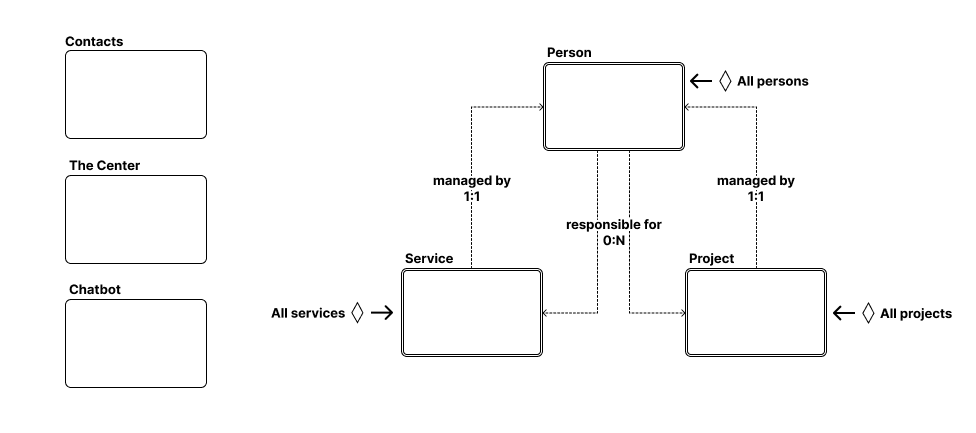
\includegraphics[width=1\linewidth]{img/design-document/C-IDM.png}
\captionof{figure}{C-IDM of The Hive's website}

\section{Content-in-the-small}
\subsection{Content Tables}
Following the C-IDM, we define more in detail the content by means of Content Tables. Detailed Abstract Pages are available in the Annex section of this document.

\vspace{2em}

\begin{center}
%Kind Of Topic: Person
\begin{tabular}{ |p{5cm}|p{6cm}| }
    \rowcolor{gray}
    \hline
    \multicolumn{2}{|l|}{\textbf{KIND OF TOPIC: Person}} \\
    \hline
    Person Name & text \\
    \hline
    Person Education & text \\
    \hline
    Person Main Expertise & text \\
    \hline
    Person Main Role & text \\
    \hline
    List of Managed Activities & [Service Name, Project Name]\\
    \hline
\end{tabular}

\vspace{2em}
%Kind Of Topic: Service
\begin{tabular}{ |p{5cm}|p{6cm}| }
    \rowcolor{gray}
    \hline
    \multicolumn{2}{|l|}{\textbf{KIND OF TOPIC: Service}} \\
    \hline
    Service Name & text \\
    \hline
    Service Responsible & Person Name \\
    \hline
    Service Date & Date \\
    \hline
    Service Description & text \\
    \hline
    List of Testimonials & [User Name, User Image, User Text] \\
    \hline
\end{tabular}

\vspace{2em}
%Kind Of Topic: Project
\begin{tabular}{ |p{5cm}|p{6cm}| }
    \rowcolor{gray}
    \hline
    \multicolumn{2}{|l|}{\textbf{KIND OF TOPIC: Project}} \\
    \hline
    Project Name & text \\
    \hline
    Project Responsible & Person Name \\
    \hline
    Project Starting Date & date \\
    \hline
    Project Logo & image \\
    \hline
    Project Description & text\\
    \hline
\end{tabular}

\vspace{2em}
%Topic: Chat Bot
\begin{tabular}{ |p{5cm}|p{6cm}| }
    \rowcolor{gray}
    \hline
    \multicolumn{2}{|l|}{\textbf{TOPIC: Chat Bot}} \\
    \hline
    User Input & text \\
    \hline
    Bot Answer & text \\
    \hline
\end{tabular}

\vspace{2em}
%Group of Topics: All Persons
\begin{tabular}{ |p{5cm}|p{6cm}| }
    \rowcolor{gray}
    \hline
    \multicolumn{2}{|l|}{\textbf{GROUP OF TOPICS: All Persons}} \\
    \hline
    Group Title & "Our Team" \\
    \hline
    People & [Person Name, Person Image, Person Role] \\
    \hline
\end{tabular}

\vspace{2em}
%Topic: Contacts
\begin{tabular}{ |p{5cm}|p{6cm}| }
    \rowcolor{gray}
    \hline
    \multicolumn{2}{|l|}{\textbf{TOPIC: Contacts}} \\
    \hline
    UsefulContacts & [Telephone Number, Name]\\
    \hline
\end{tabular}

\vspace{2em}
%Group of Topics: All Services
\begin{tabular}{ |p{5cm}|p{6cm}| }
    \rowcolor{gray}
    \hline
    \multicolumn{2}{|l|}{\textbf{GROUP OF TOPICS: All Services}} \\
    \hline
    Group Title & "Our Services" \\
    \hline
    Services & [Service Title, Service Image, Service Description] \\
    \hline
\end{tabular}

\vspace{2em}
%Group of Topics: All Projects
\begin{tabular}{ |p{5cm}|p{6cm}| }
    \rowcolor{gray}
    \hline
    \multicolumn{2}{|l|}{\textbf{GROUP OF TOPICS: All Projects}} \\
    \hline
    Group Title & "Our Projects" \\
    \hline
    Services & [Project Name, Project Image, Project Description] \\
    \hline
\end{tabular}

\end{center}


\pagebreak
\section{Final Commented Screenshots}
In this section we present the result of the navigation and presentation design. With a series of screenshots we show the general look and feel of the finished website, highlighting page and link types that we choose to implement.


%Homepage
\subsection{Homepage}
The homepage summarizes the content of the overall website. Each section introduces and links, with the respective buttons, to each specific page.
The navigation bar on top contains the landmarks necessary to navigate across different kinds of topic and topics, and call-for-actions buttons on the first landing screen
guide the user to the main points of interest of the center: Contacts and Chat Bot.
\vspace{1em}

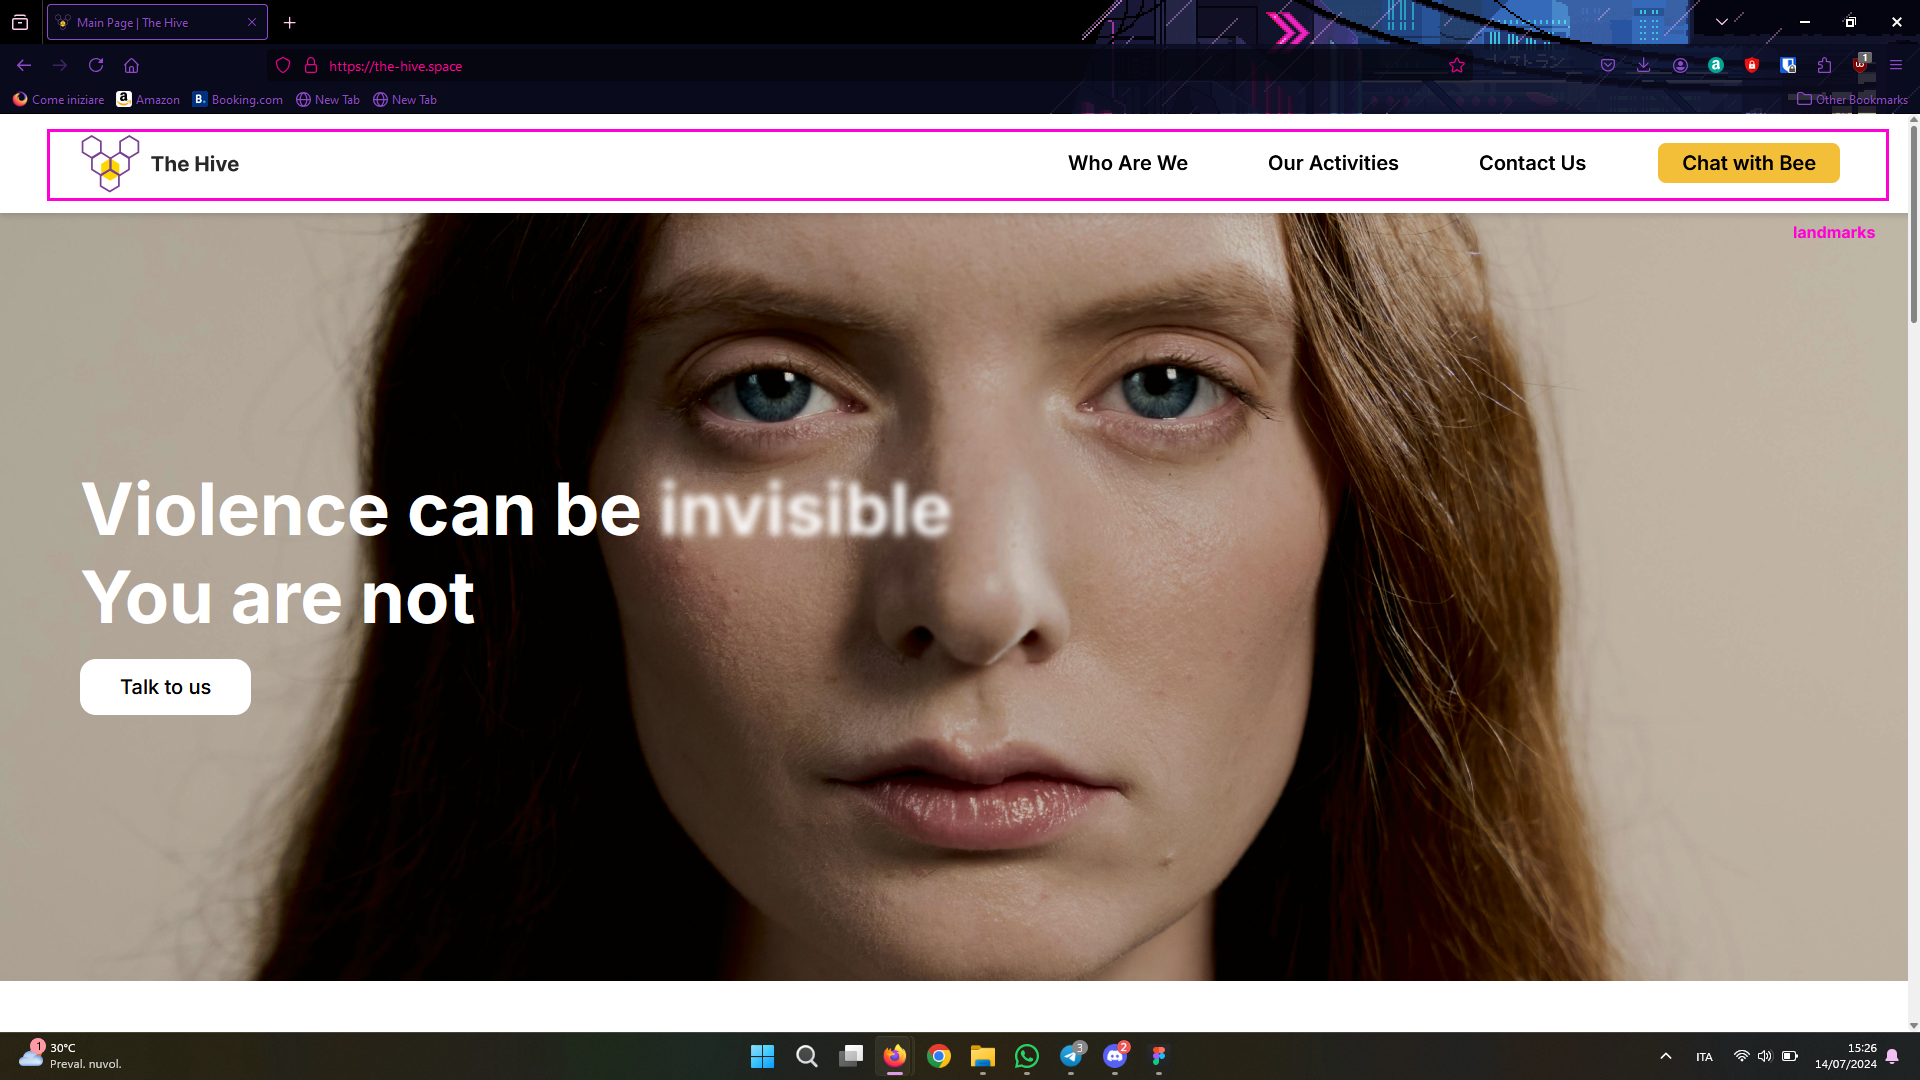
\includegraphics[width=0.5\linewidth]{img/design-document/website-screenshots/homepage-1.png}
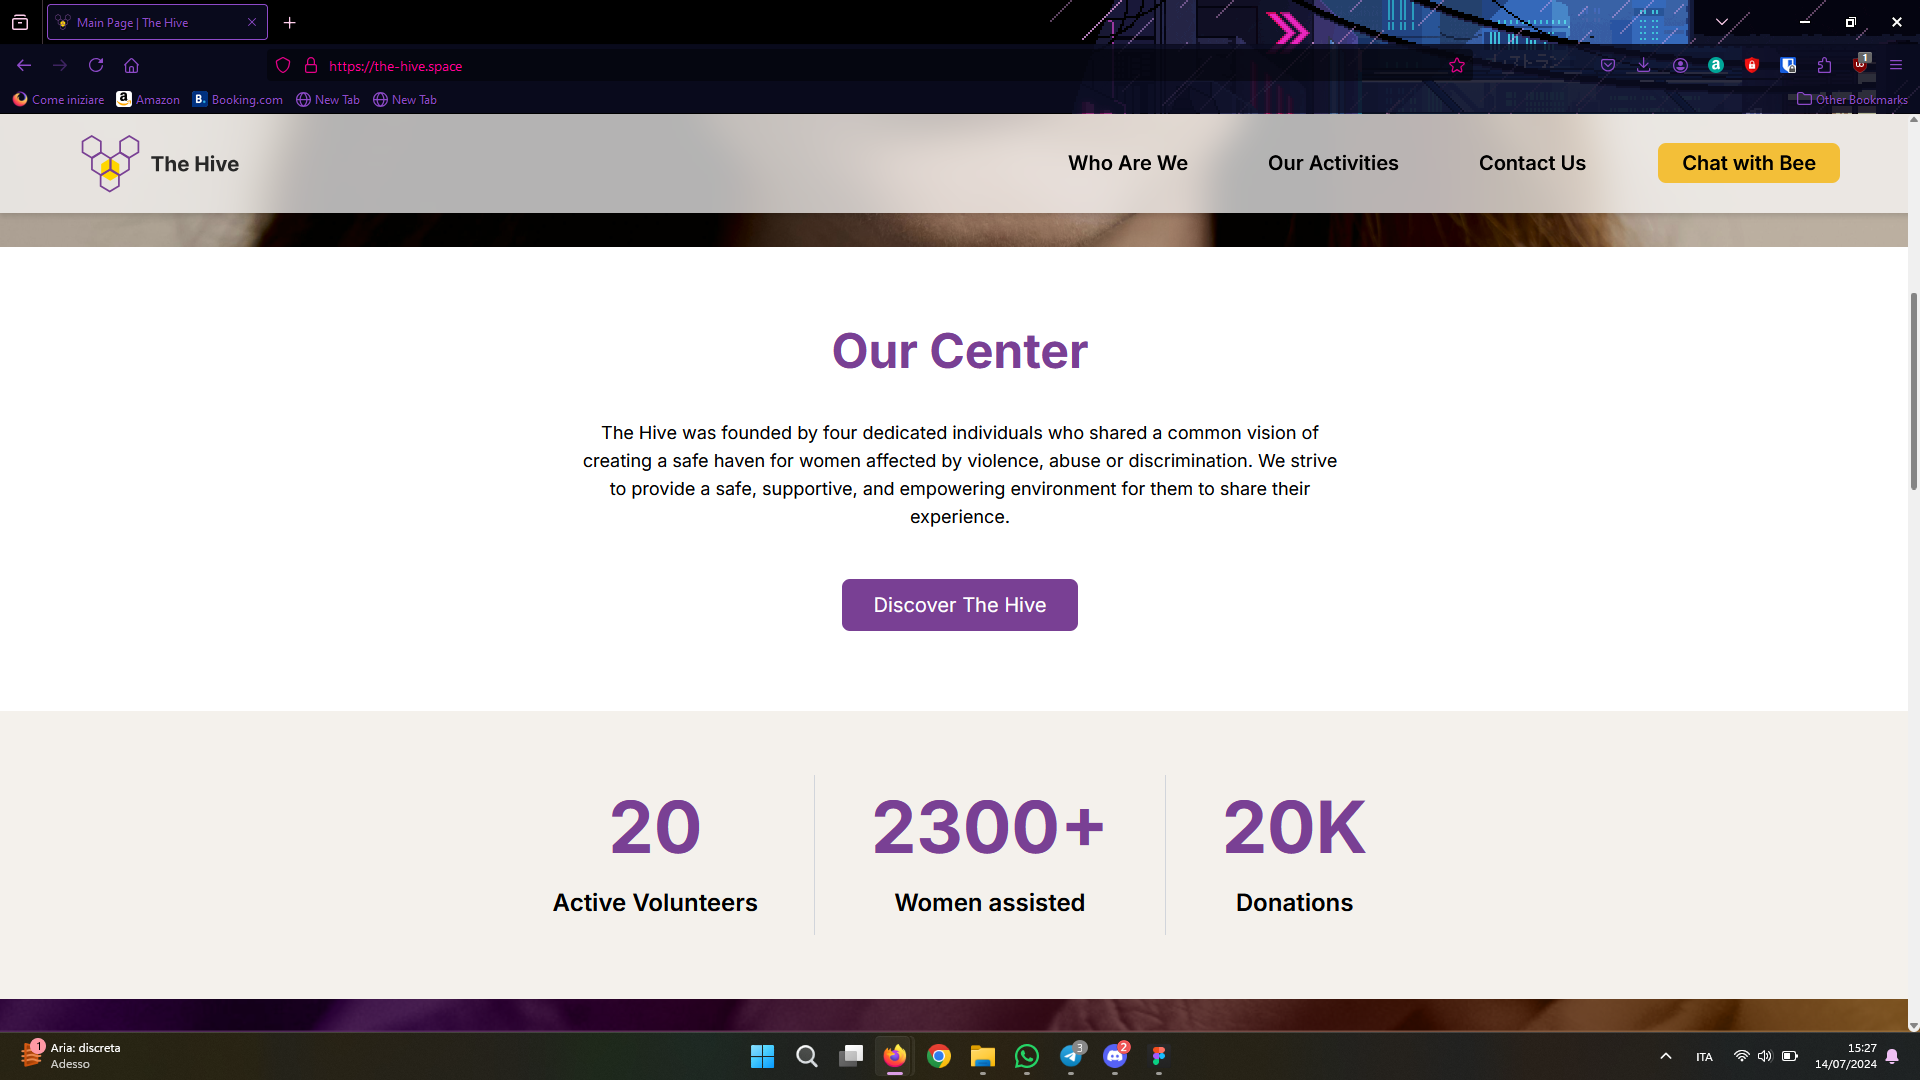
\includegraphics[width=0.5\linewidth]{img/design-document/website-screenshots/homepage-2.png}
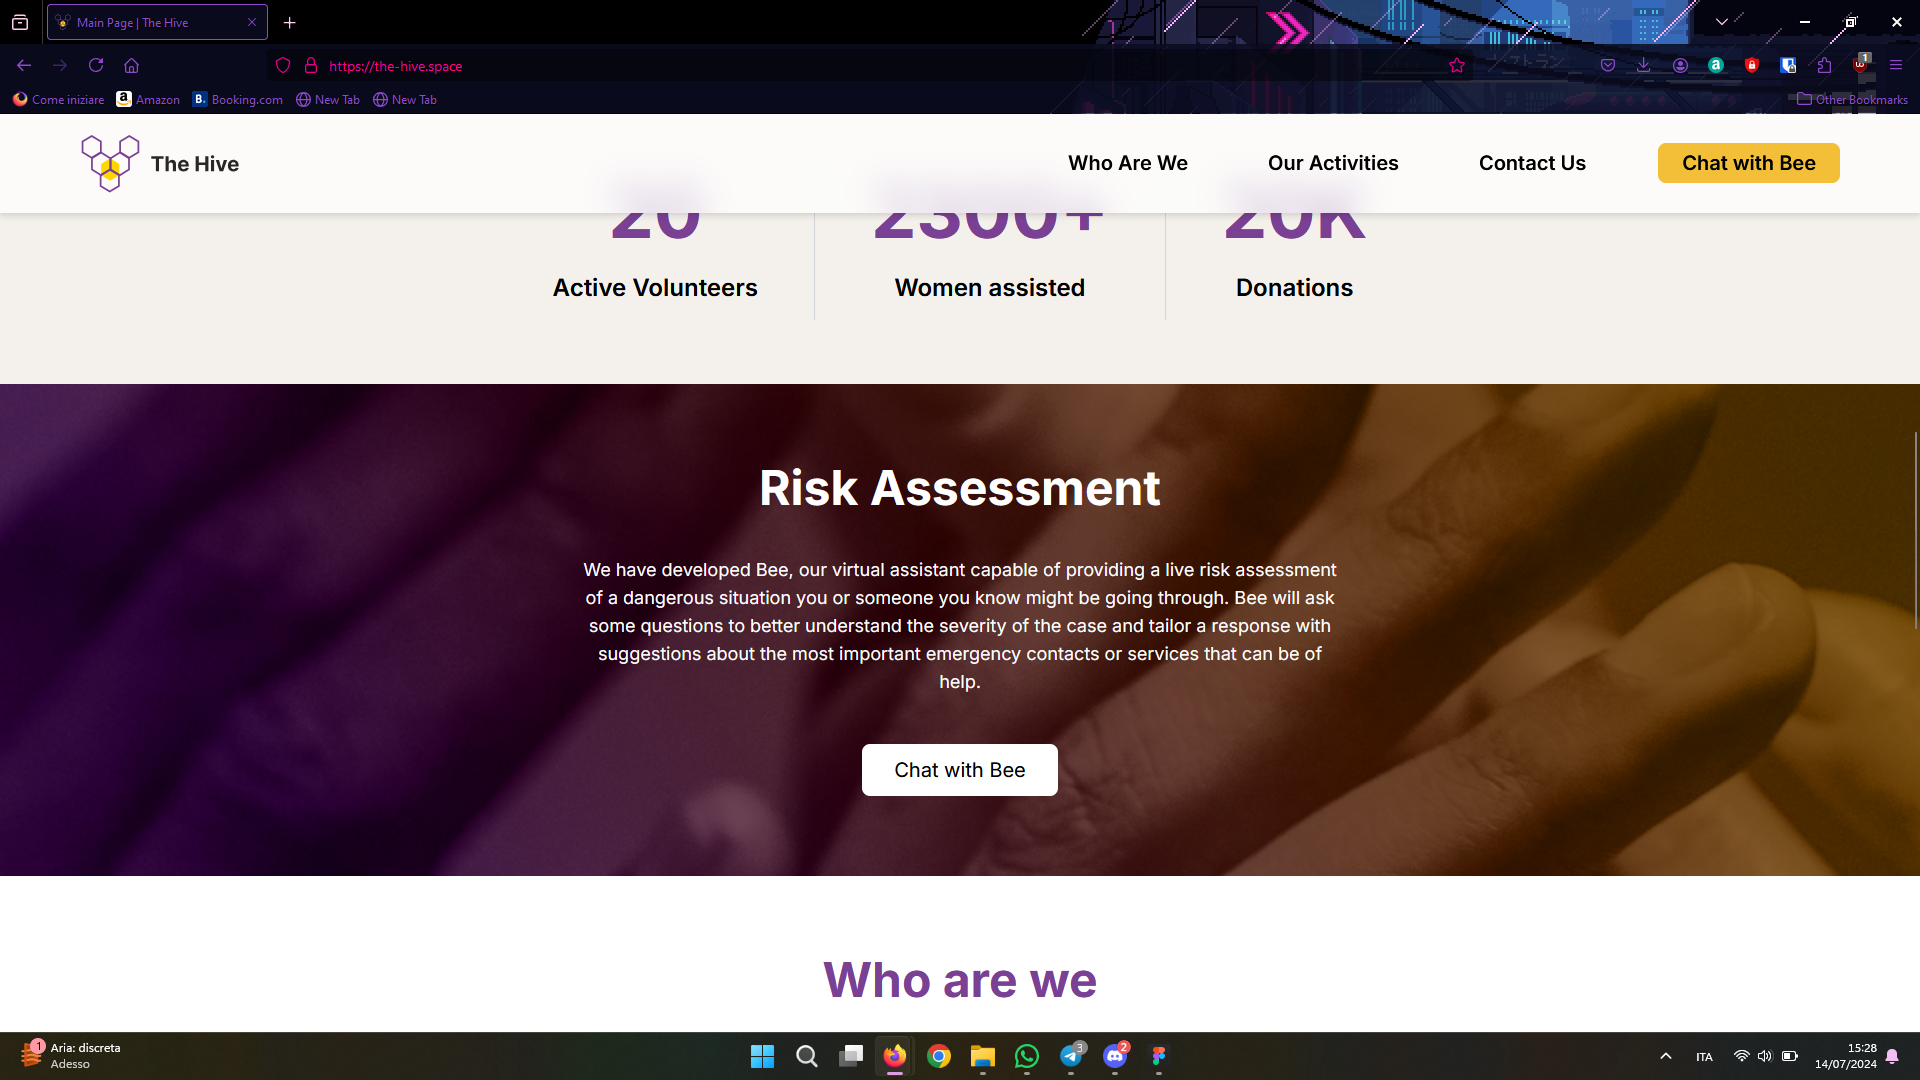
\includegraphics[width=0.5\linewidth]{img/design-document/website-screenshots/homepage-3.png}
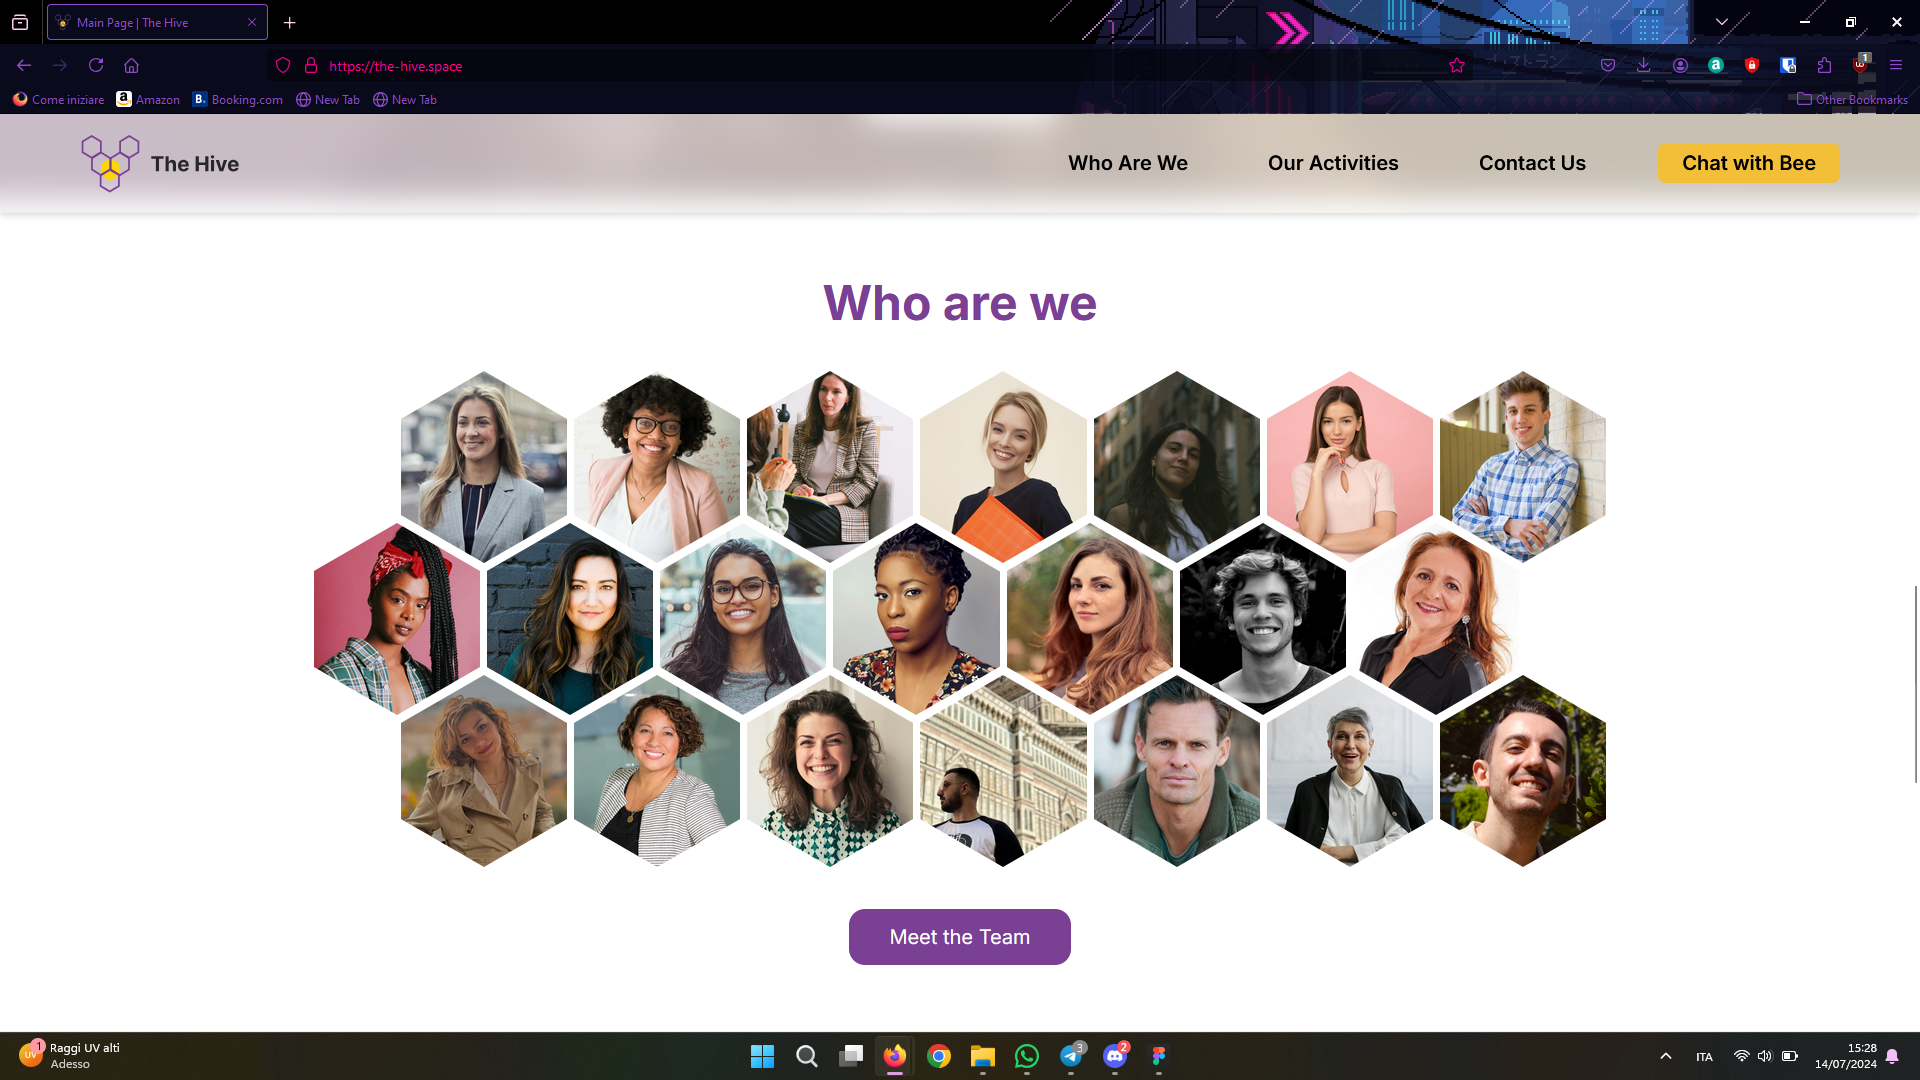
\includegraphics[width=0.5\linewidth]{img/design-document/website-screenshots/homepage-4.png}
\begin{center}
    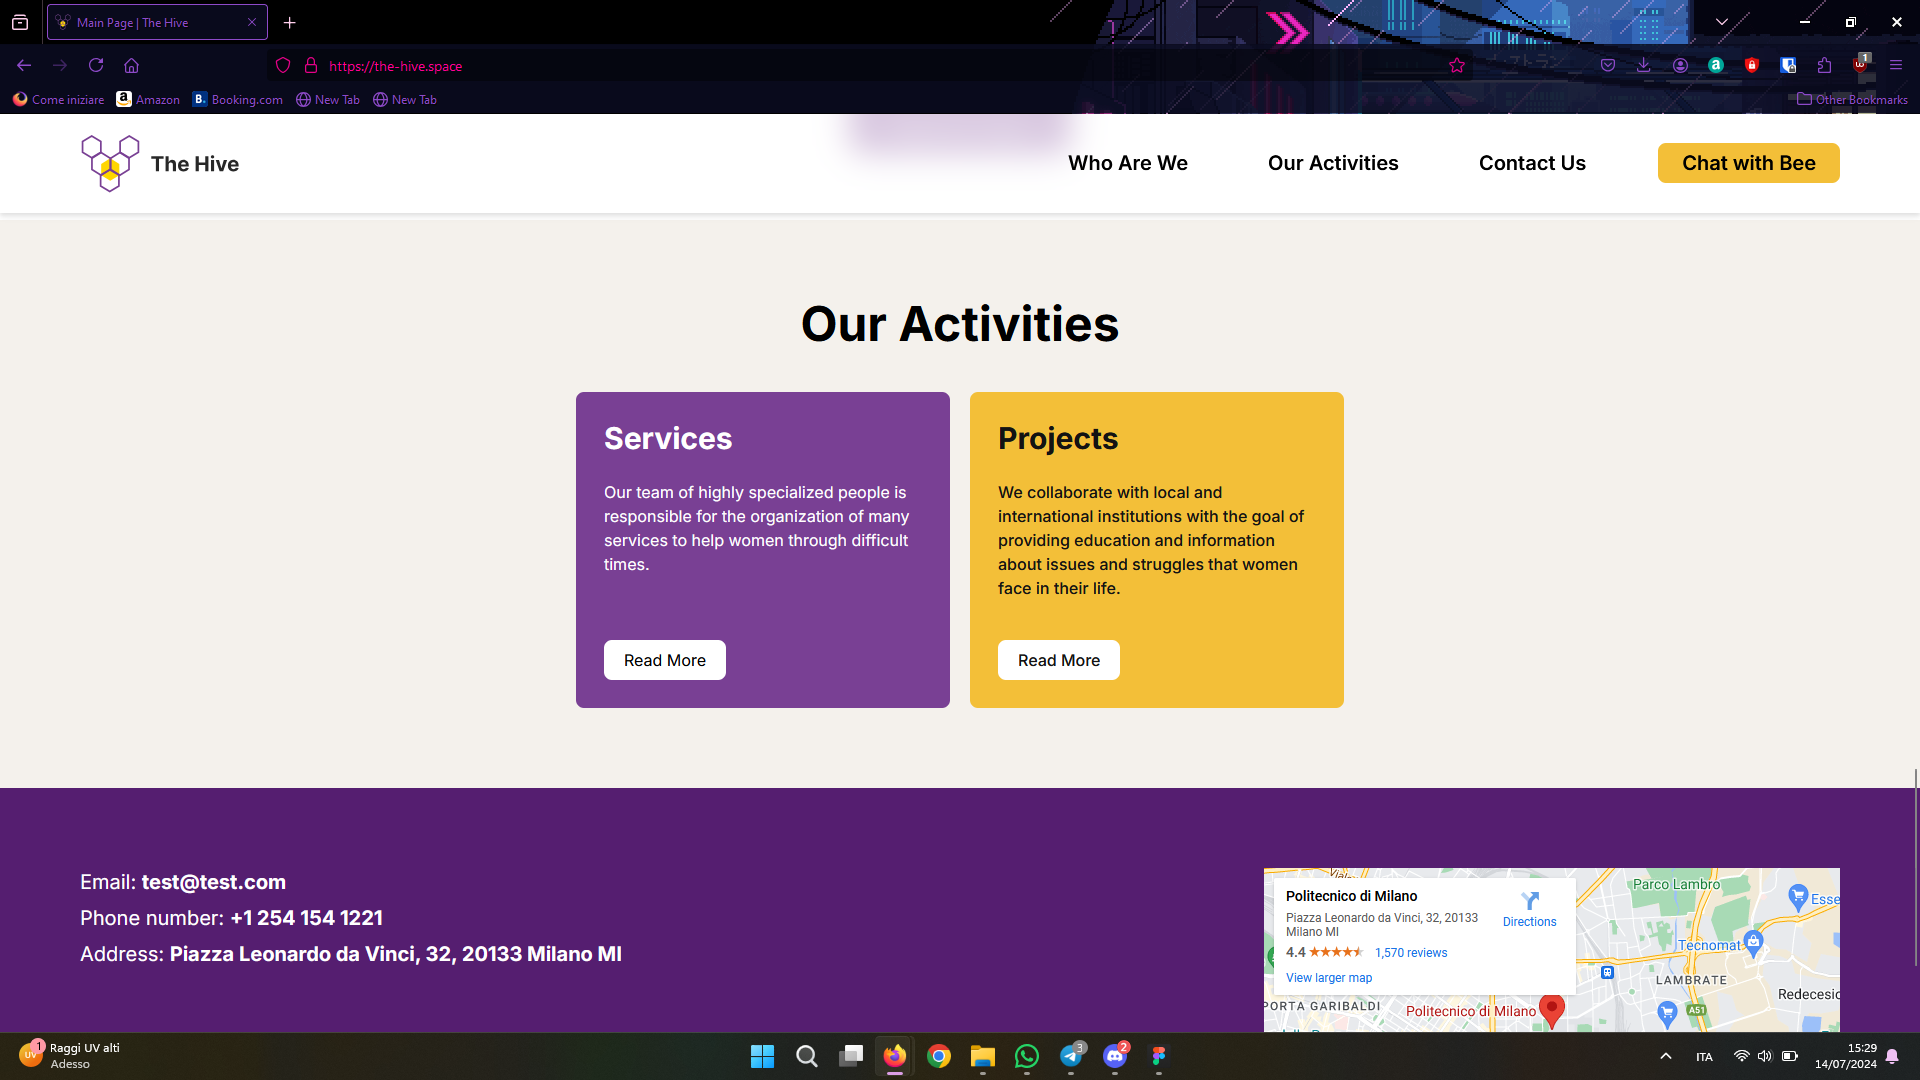
\includegraphics[width=0.5\linewidth]{img/design-document/website-screenshots/homepage-5.png}   
\end{center}

%About The Center
\subsection{The Center}
The About page of the center provides the story and mission of The Hive.
\vspace{1em}
\begin{center}
    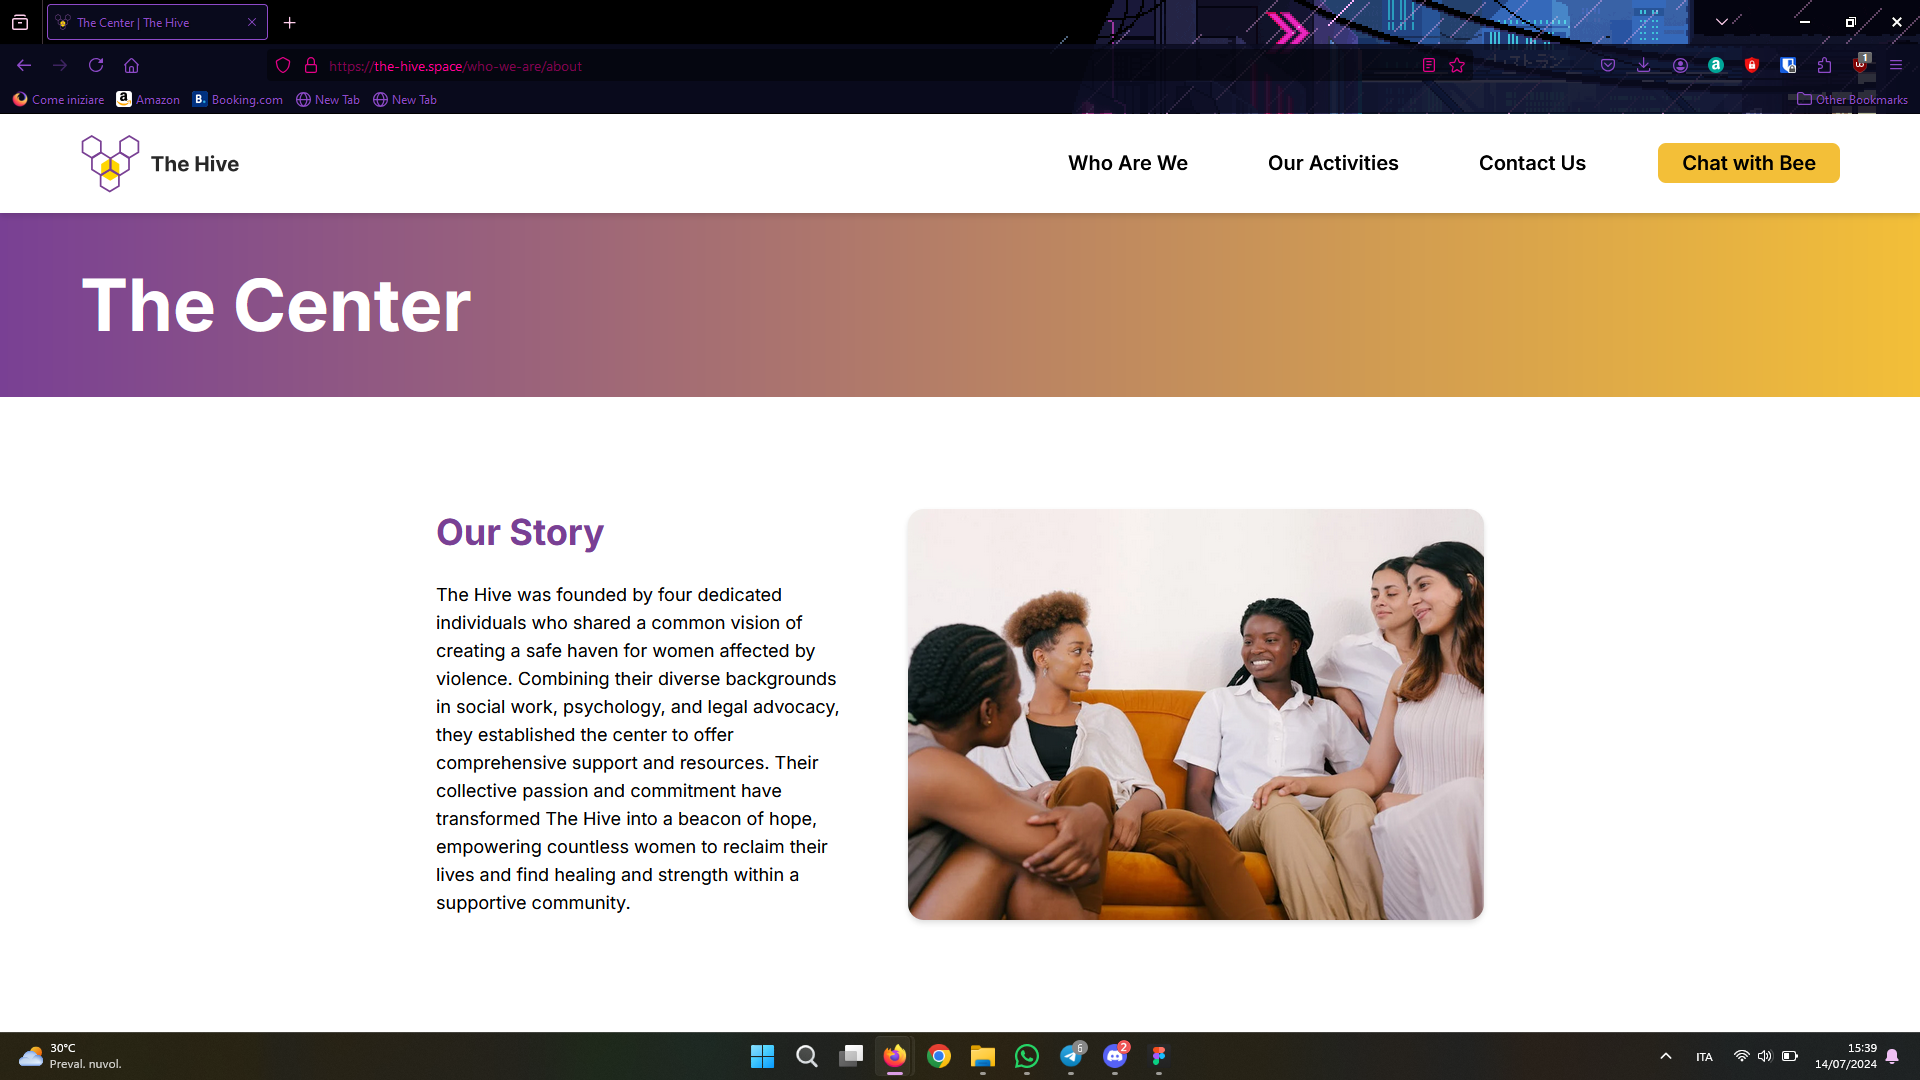
\includegraphics[width=0.5\linewidth]{img/design-document/website-screenshots/centerpage.png}   
\end{center}

%Our Team + Single Person
\subsection{Our Team}
This page collects all the people involved in The Hive. Each person is represented with their picture, name and role,
and is a group link to the single profile page. This more detailed page presents a short CV of the person with informationa
about their education, main role and expertise and a list of the activities (services and/or projects) that they are responsible for.
The links on the right are structural links that bring you to the respective anchor point, while the names of the activities 
are transition links to the specific activity. Finally, breadcrumbs are group links that bring back to the group of topic the kind of topic is part of.

\vspace{1em}
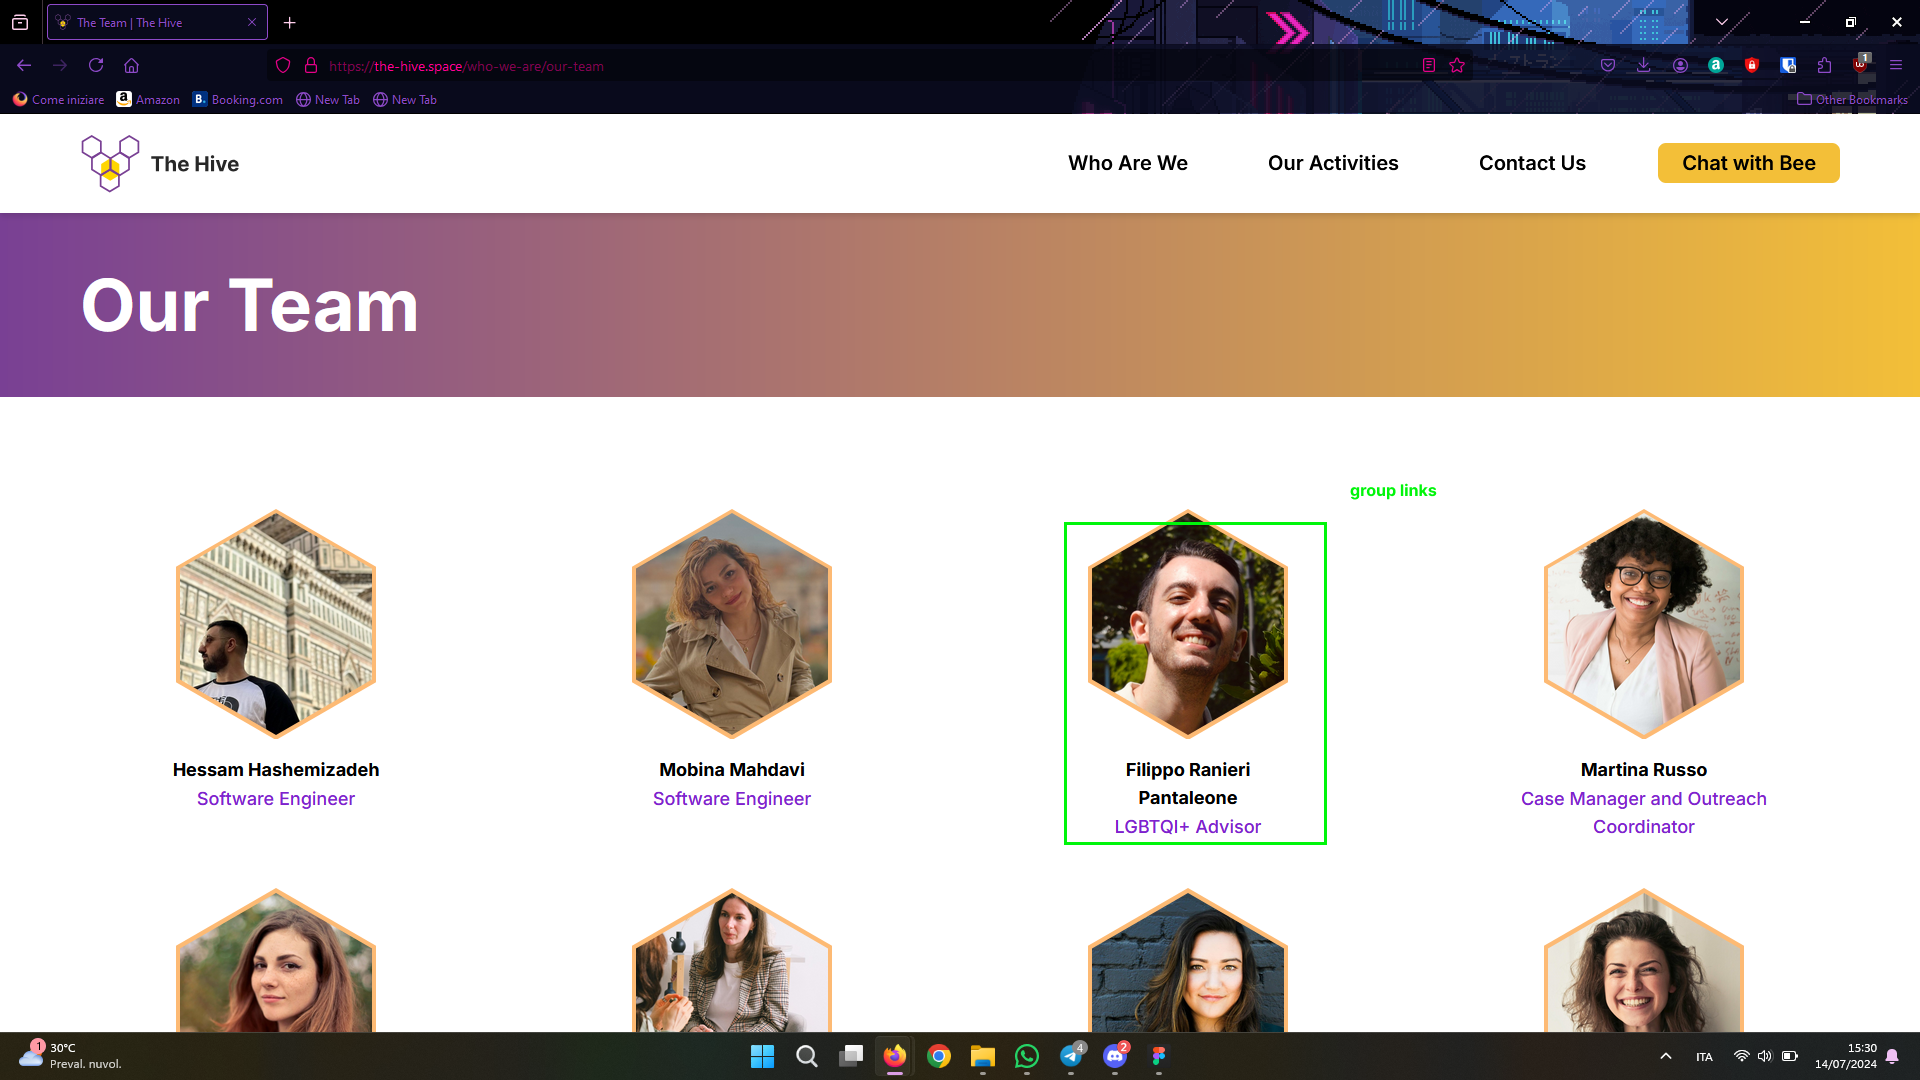
\includegraphics[width=0.5\linewidth]{img/design-document/website-screenshots/teampage.png}
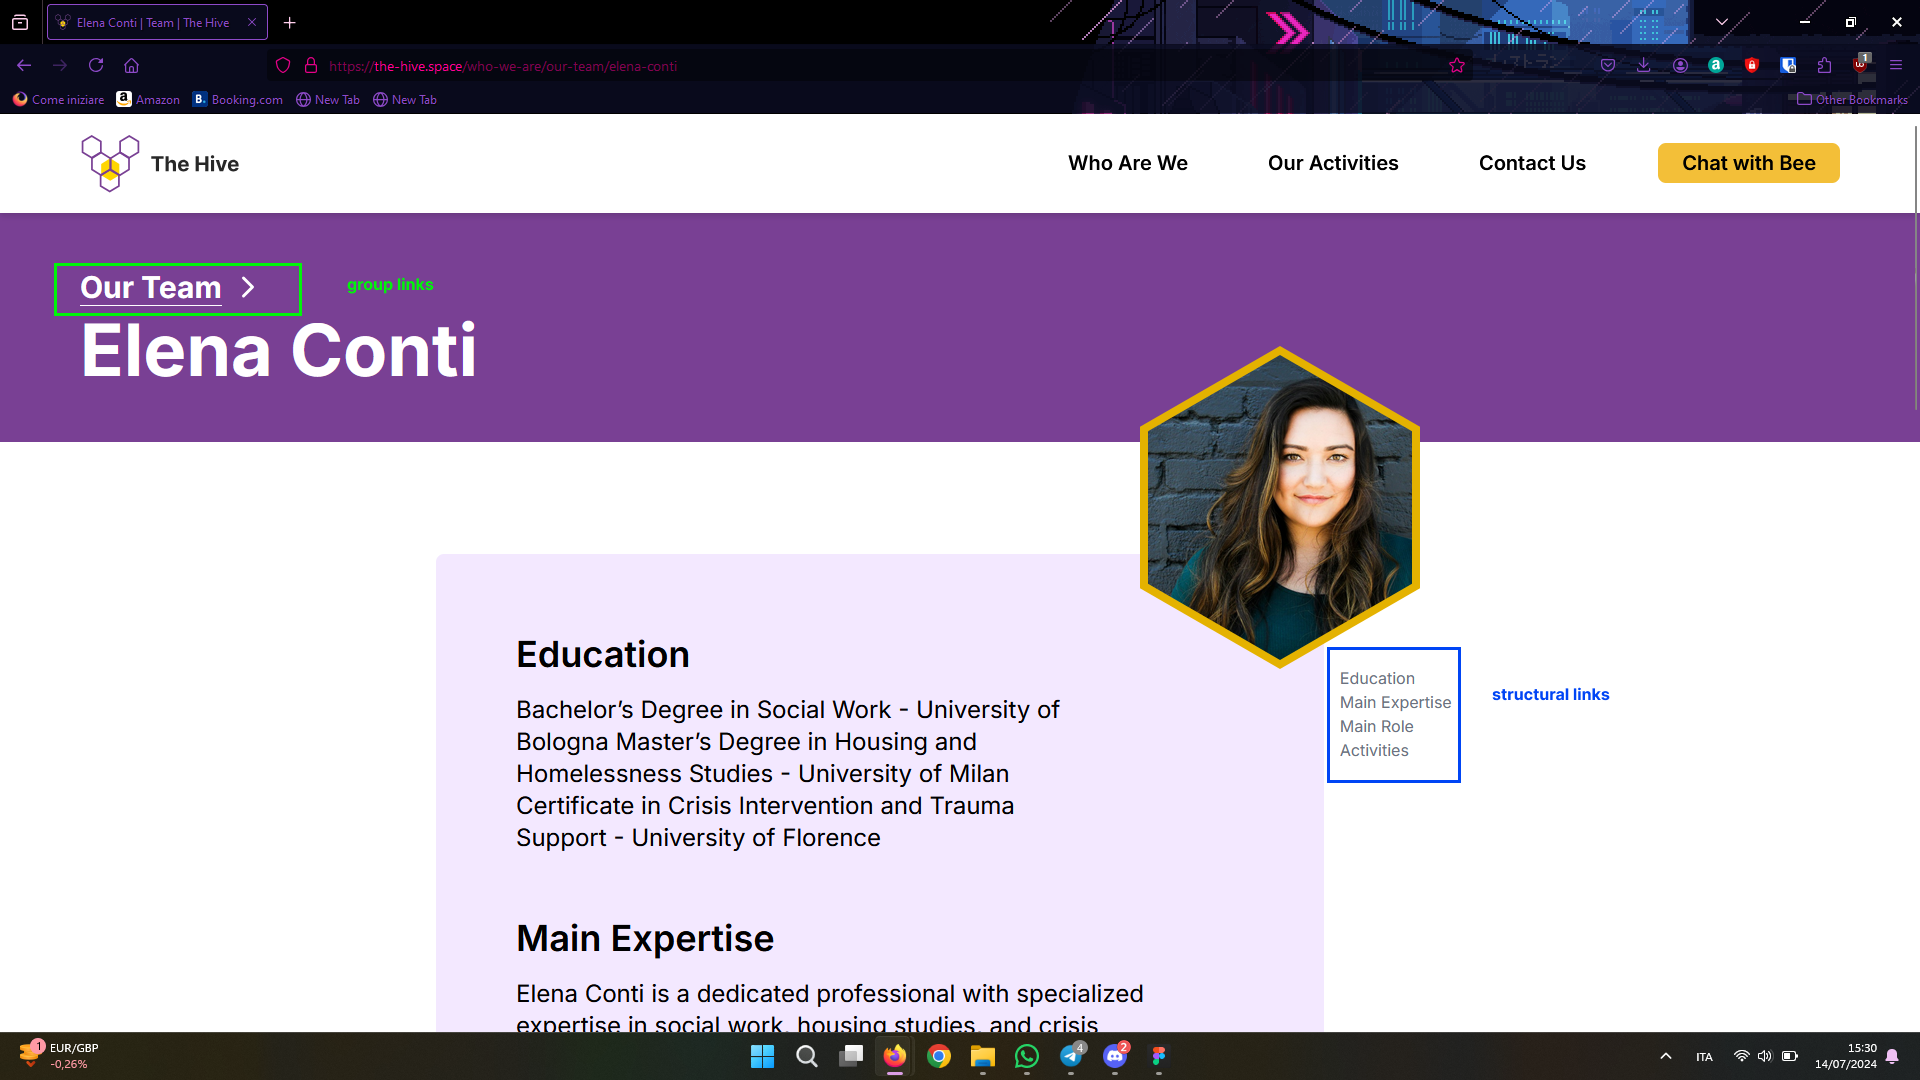
\includegraphics[width=0.5\linewidth]{img/design-document/website-screenshots/personpage-1.png}
\begin{center}
    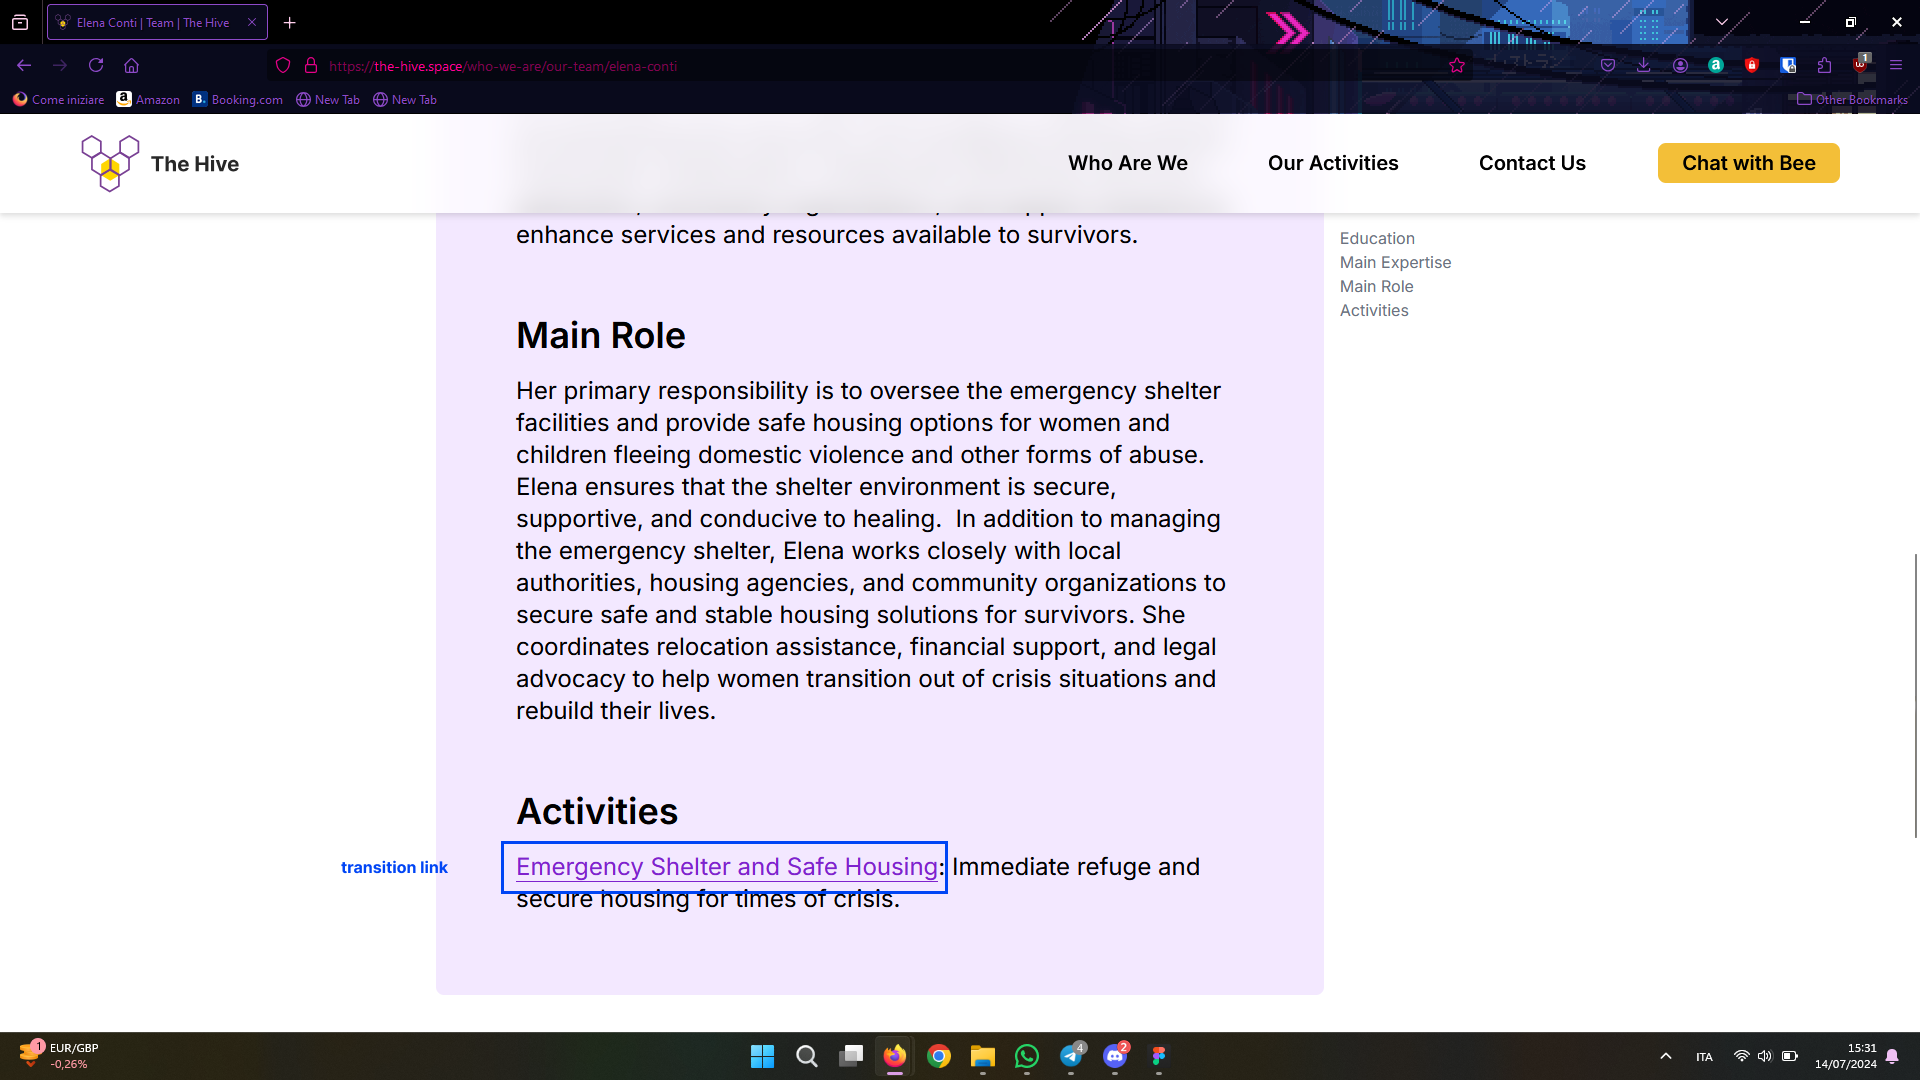
\includegraphics[width=0.5\linewidth]{img/design-document/website-screenshots/personpage-2.png}
\end{center}

%Our Services + Single Service
\subsection{Services}
This page collects all the services provided by The Hive. Each service is represented with their logo, title and short description,
and has a group link (Read More) to the single service page. This more detailed page presents a longer description of the service, the schedule and 
the name of its responsible, which is a transiction link to their profile. Furthermore, each service has a list of a couple of testimonies of people
participated in them, characterized by the User Picture, Name and Message.

\vspace{1em}
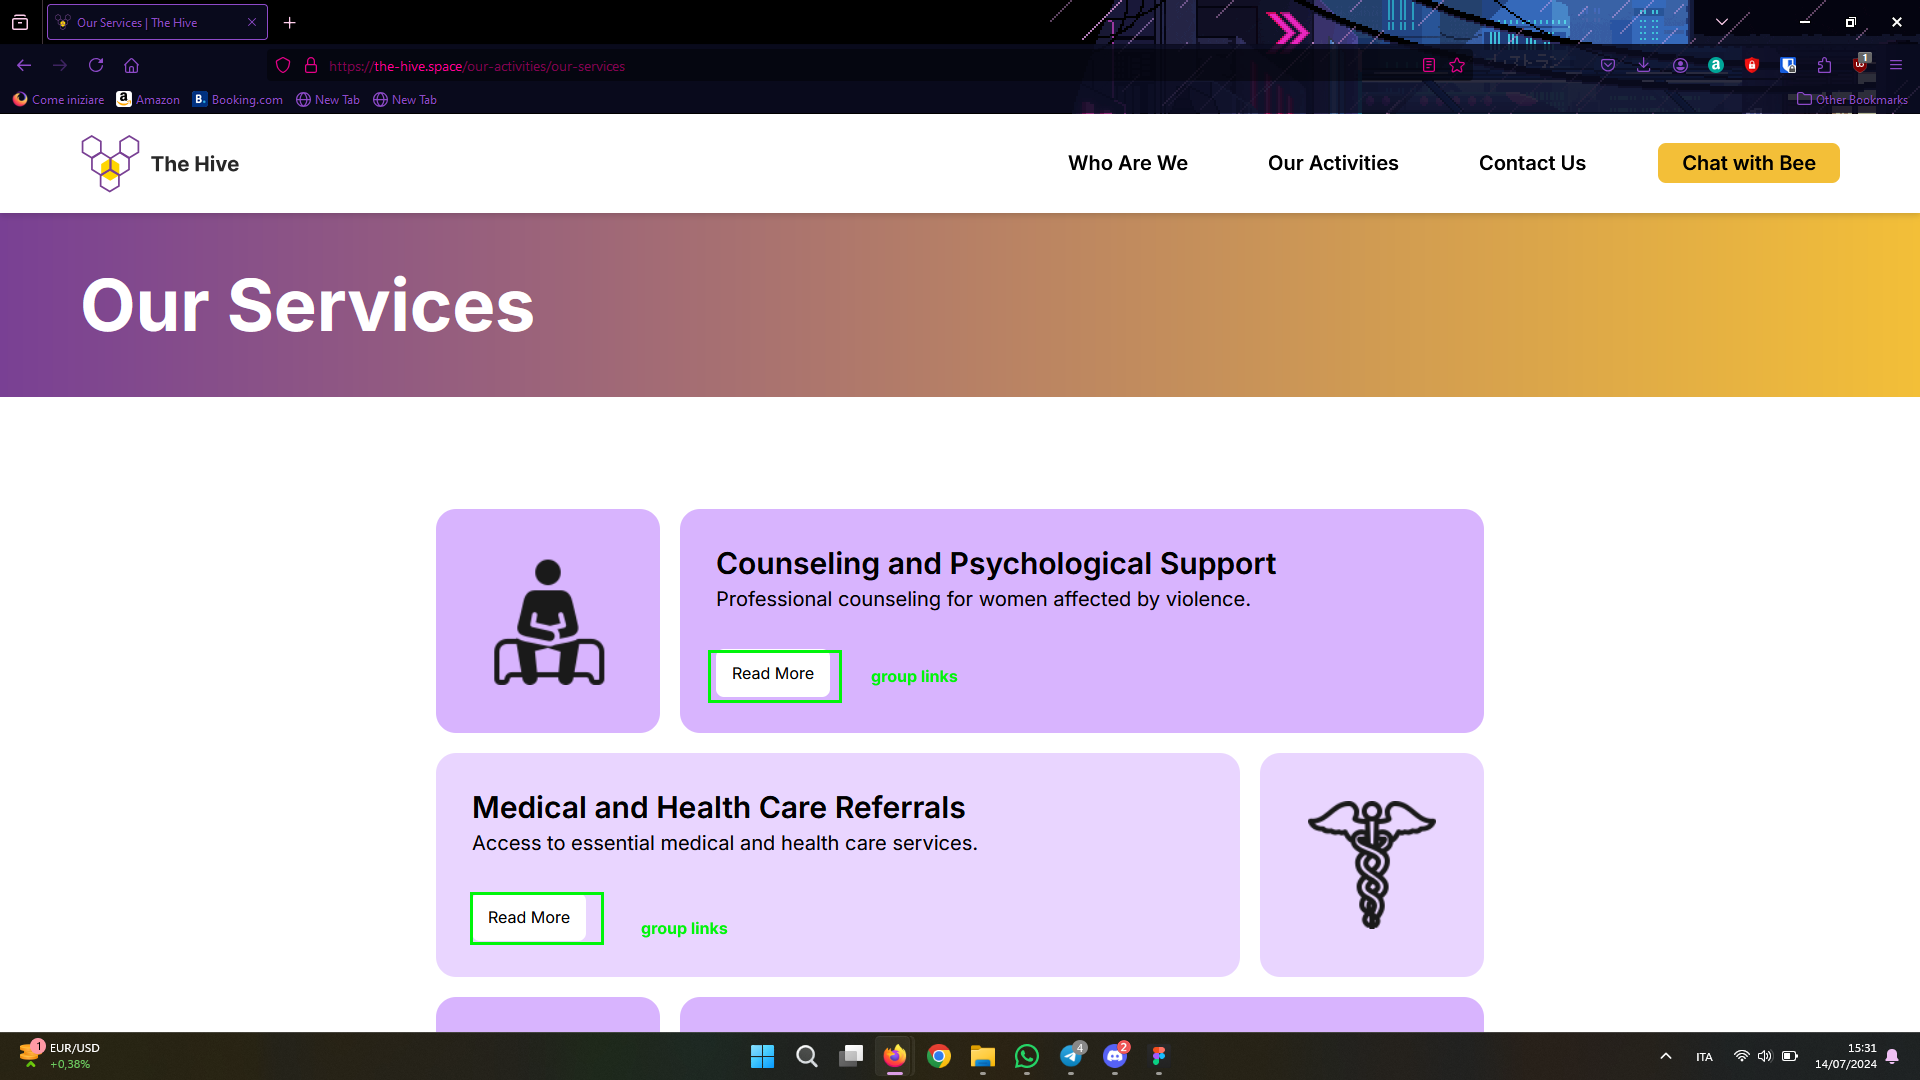
\includegraphics[width=0.5\linewidth]{img/design-document/website-screenshots/servicespage.png}
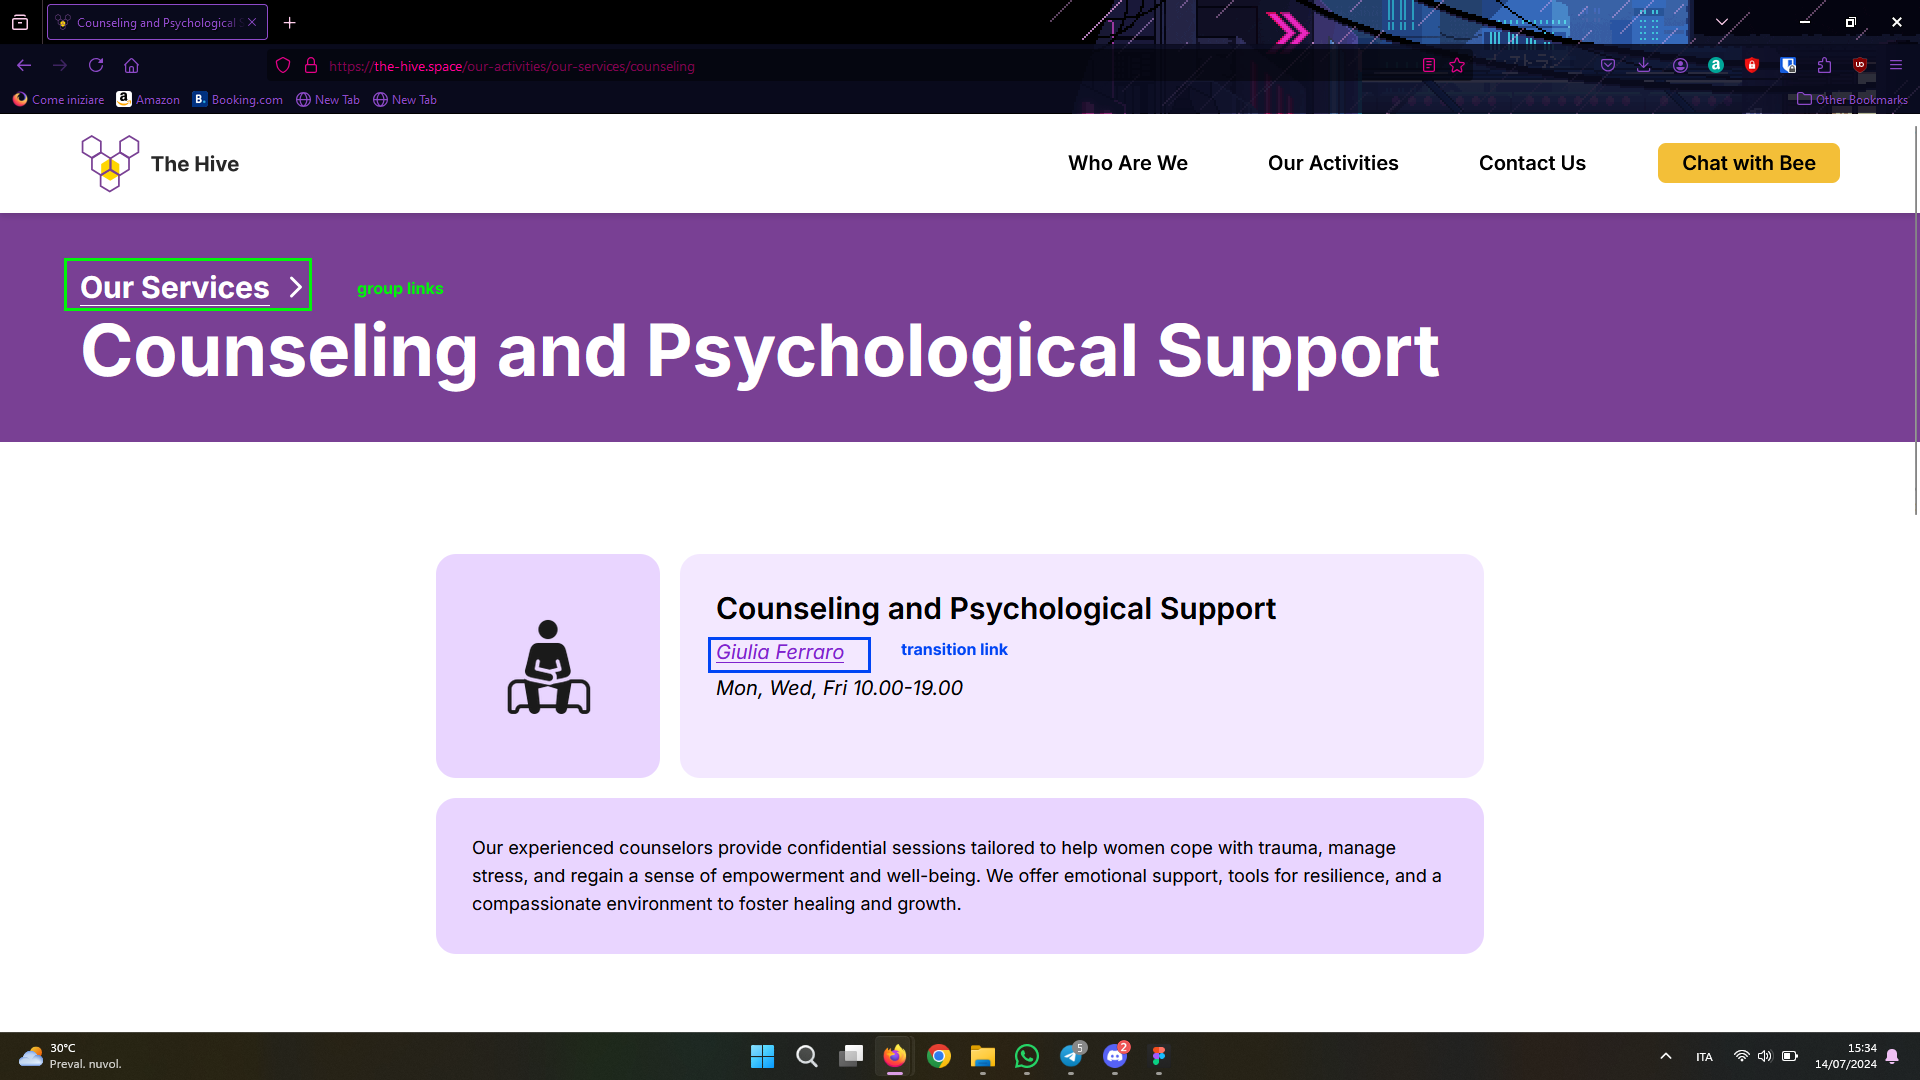
\includegraphics[width=0.5\linewidth]{img/design-document/website-screenshots/servicepage-1.png}
\begin{center}
    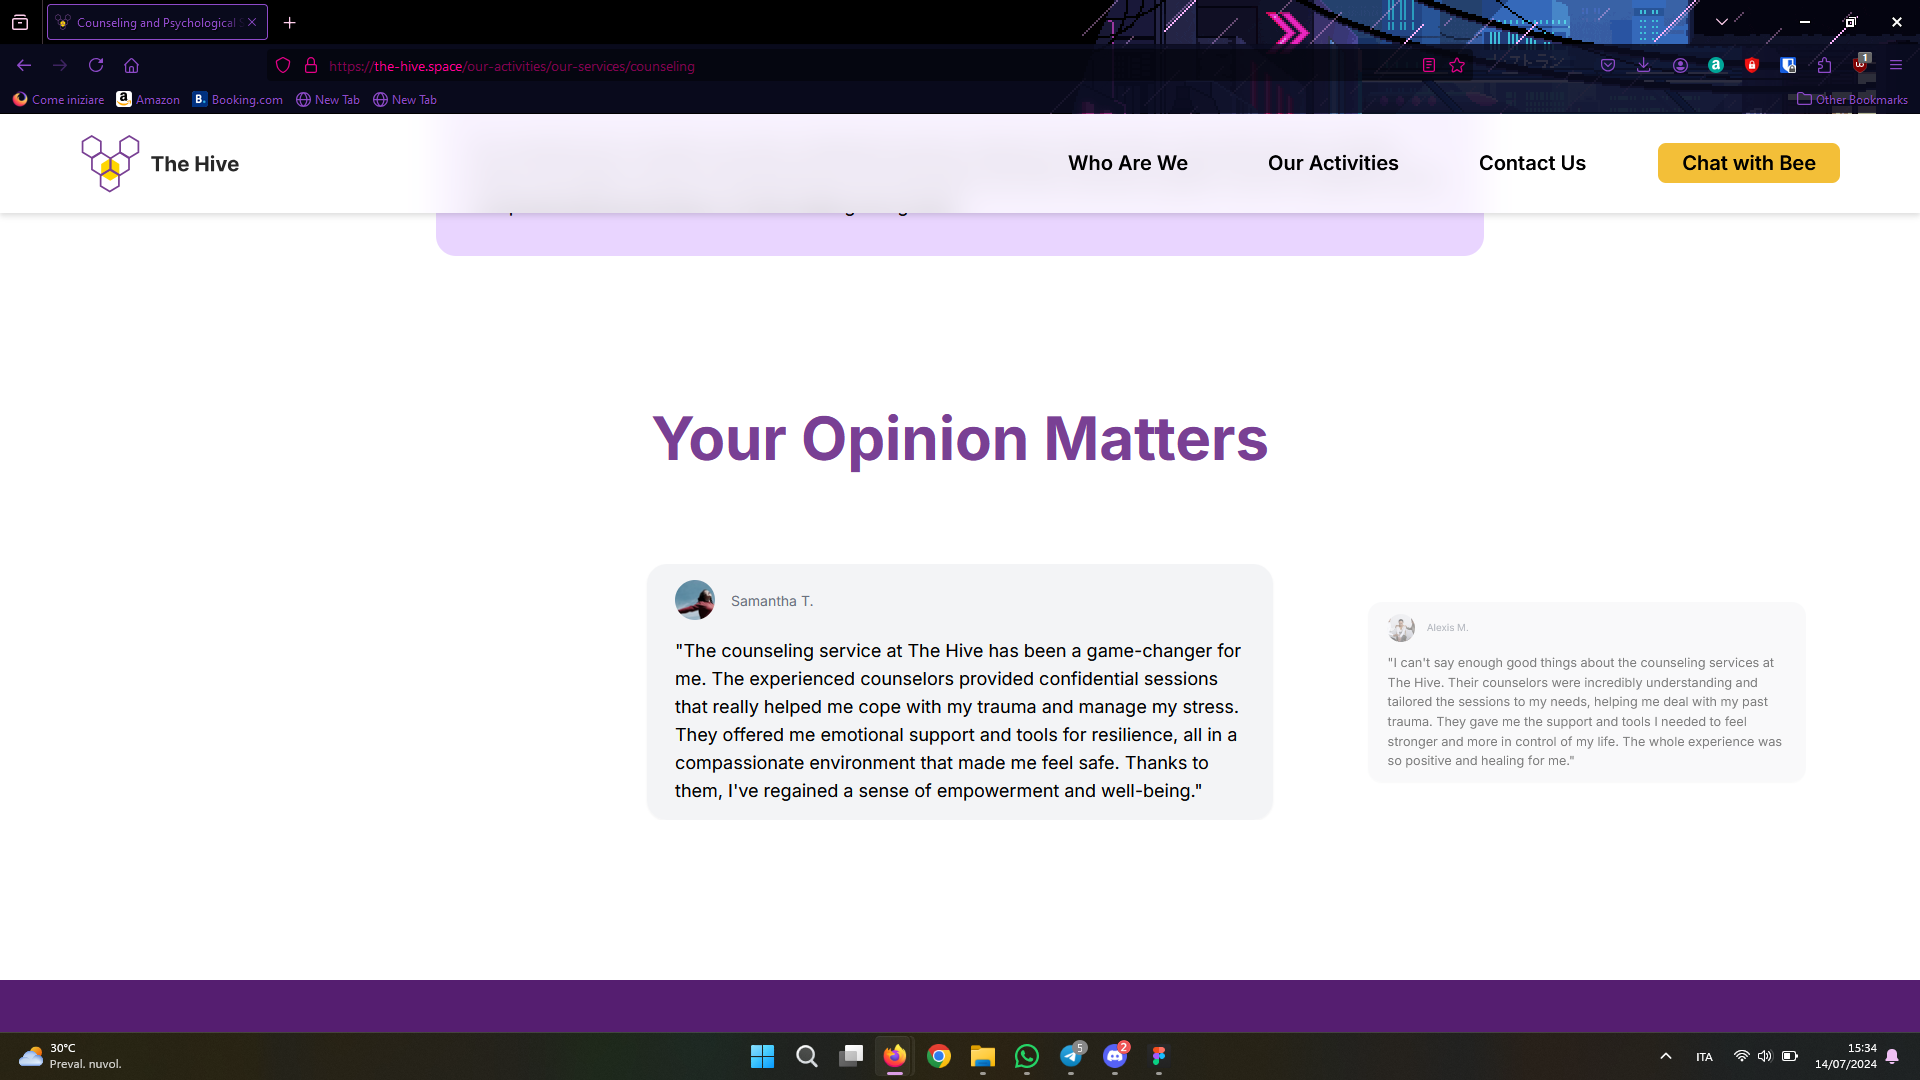
\includegraphics[width=0.5\linewidth]{img/design-document/website-screenshots/servicepage-2.png}   
\end{center}

%Our Projects + Single Project
\subsection{Our Projects}
This page collects all the projects The Hive is involved in. Each project is represented with a Picture, Title and Short Description,
and has a group link (Read More) to the single project page. This more detailed page presents a longer article about the Project, the Starting Date and 
the name of its Responsible, which is a transiction link to their profile.

\vspace{1em}
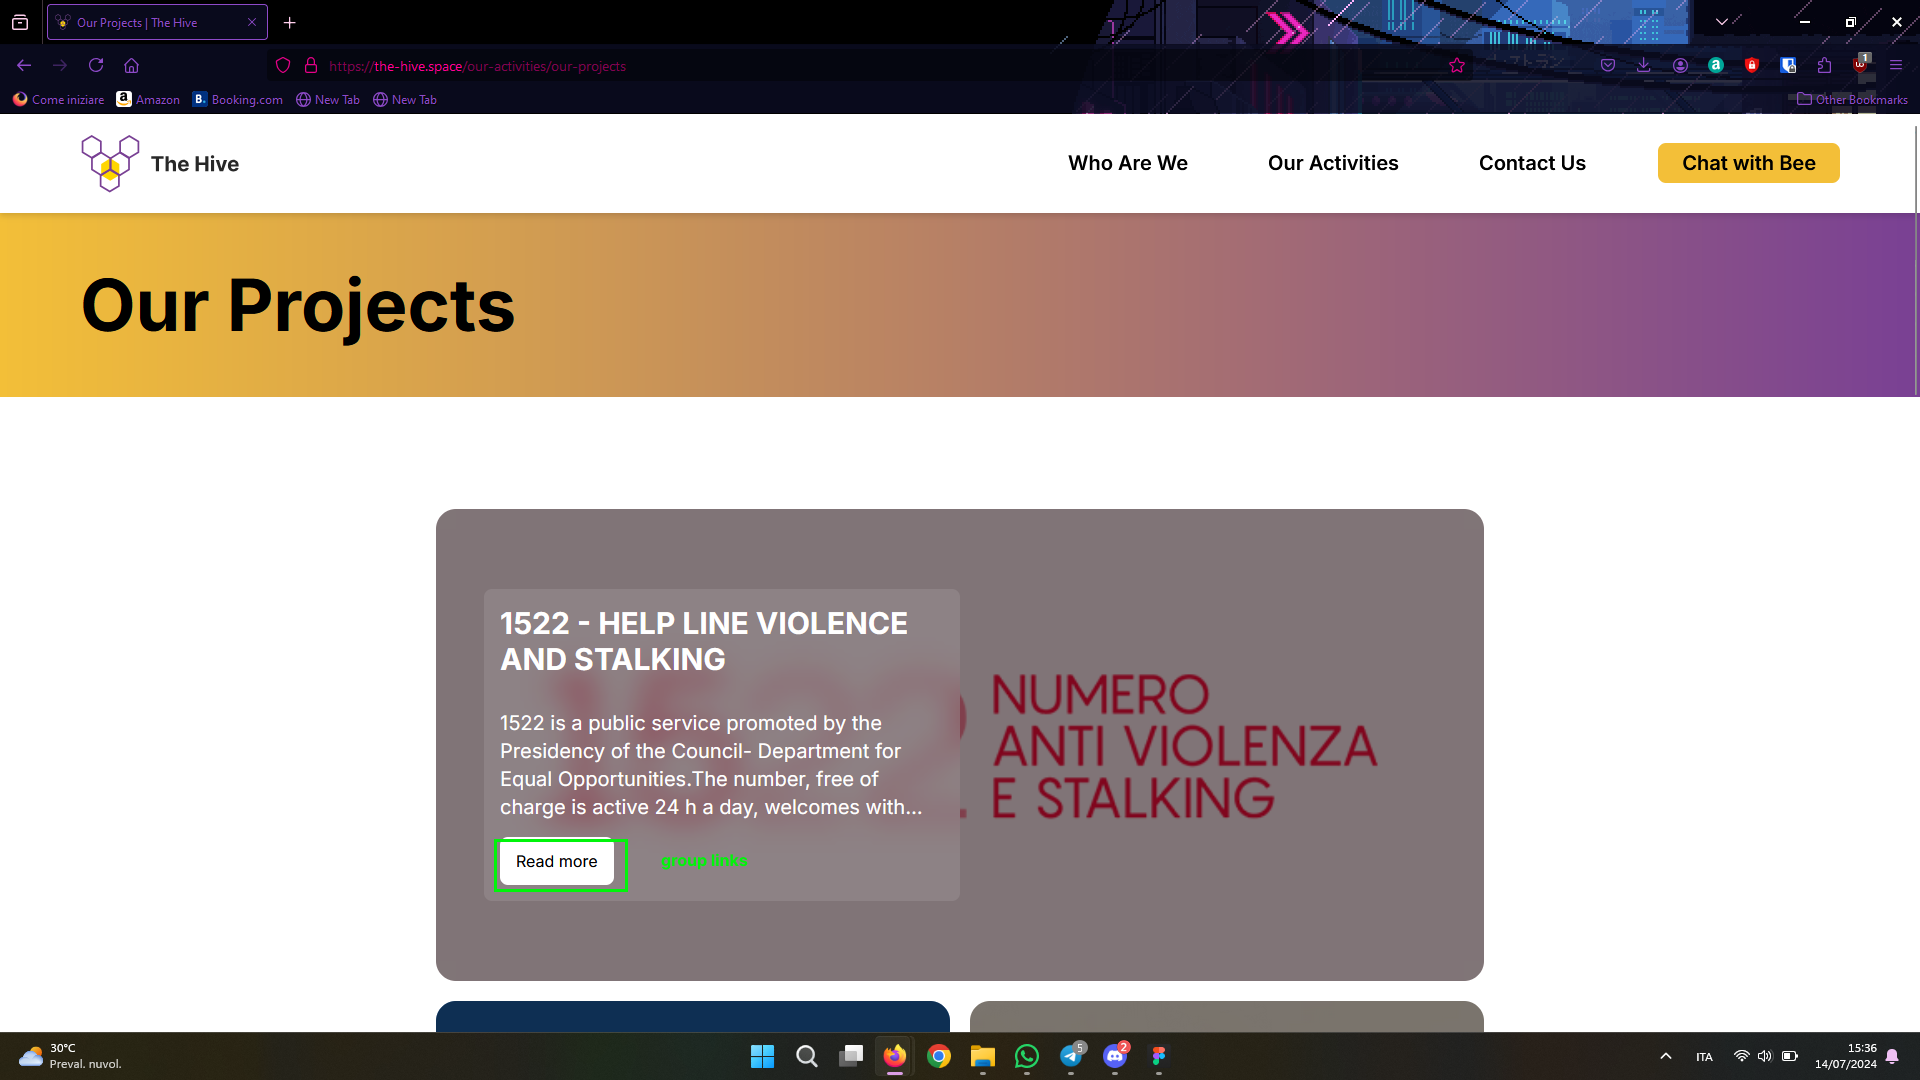
\includegraphics[width=0.5\linewidth]{img/design-document/website-screenshots/projectspage.png}
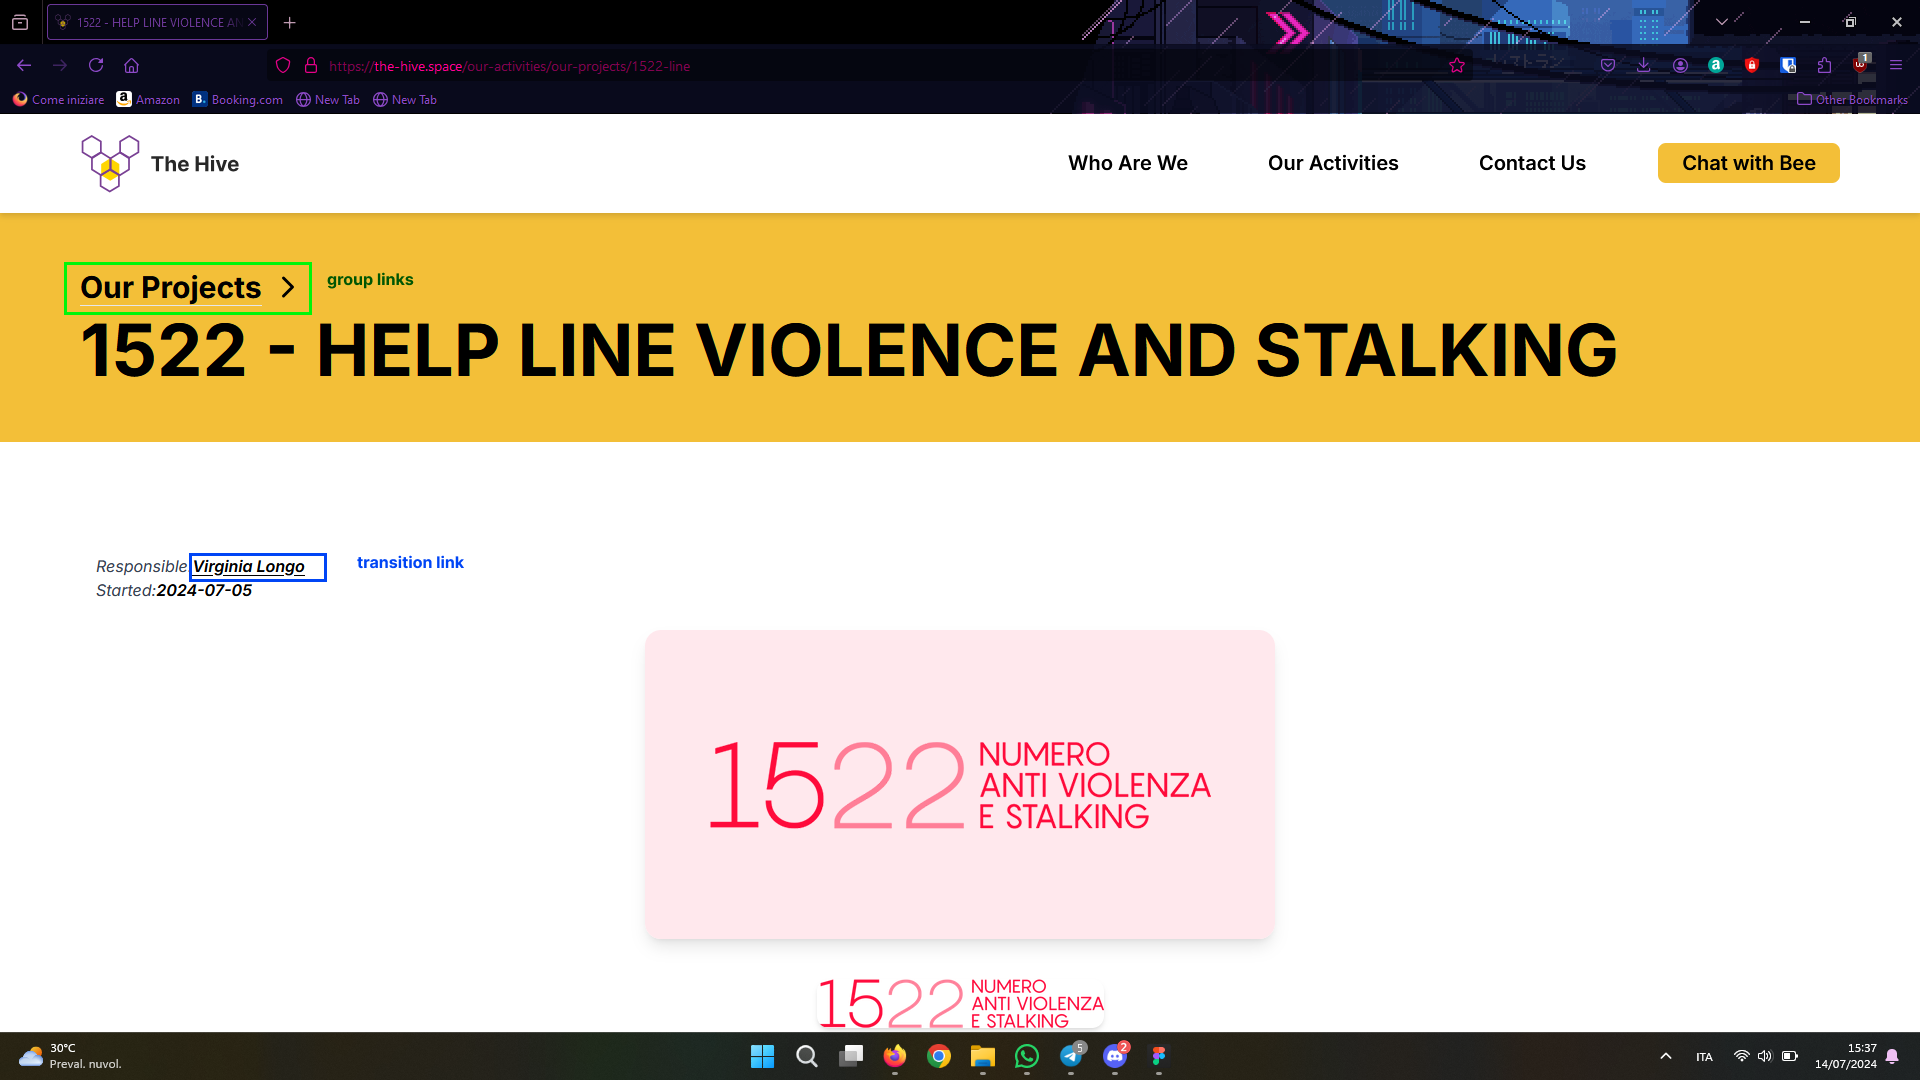
\includegraphics[width=0.5\linewidth]{img/design-document/website-screenshots/projectpage-1.png}

%Contacts
\subsection{Contacts}
The Contacts page contains some information about contacting the center, some Telephone Number of National Services and of the center itself and a 
form to send emails to contact the center.
\vspace{1em}
\begin{center}
    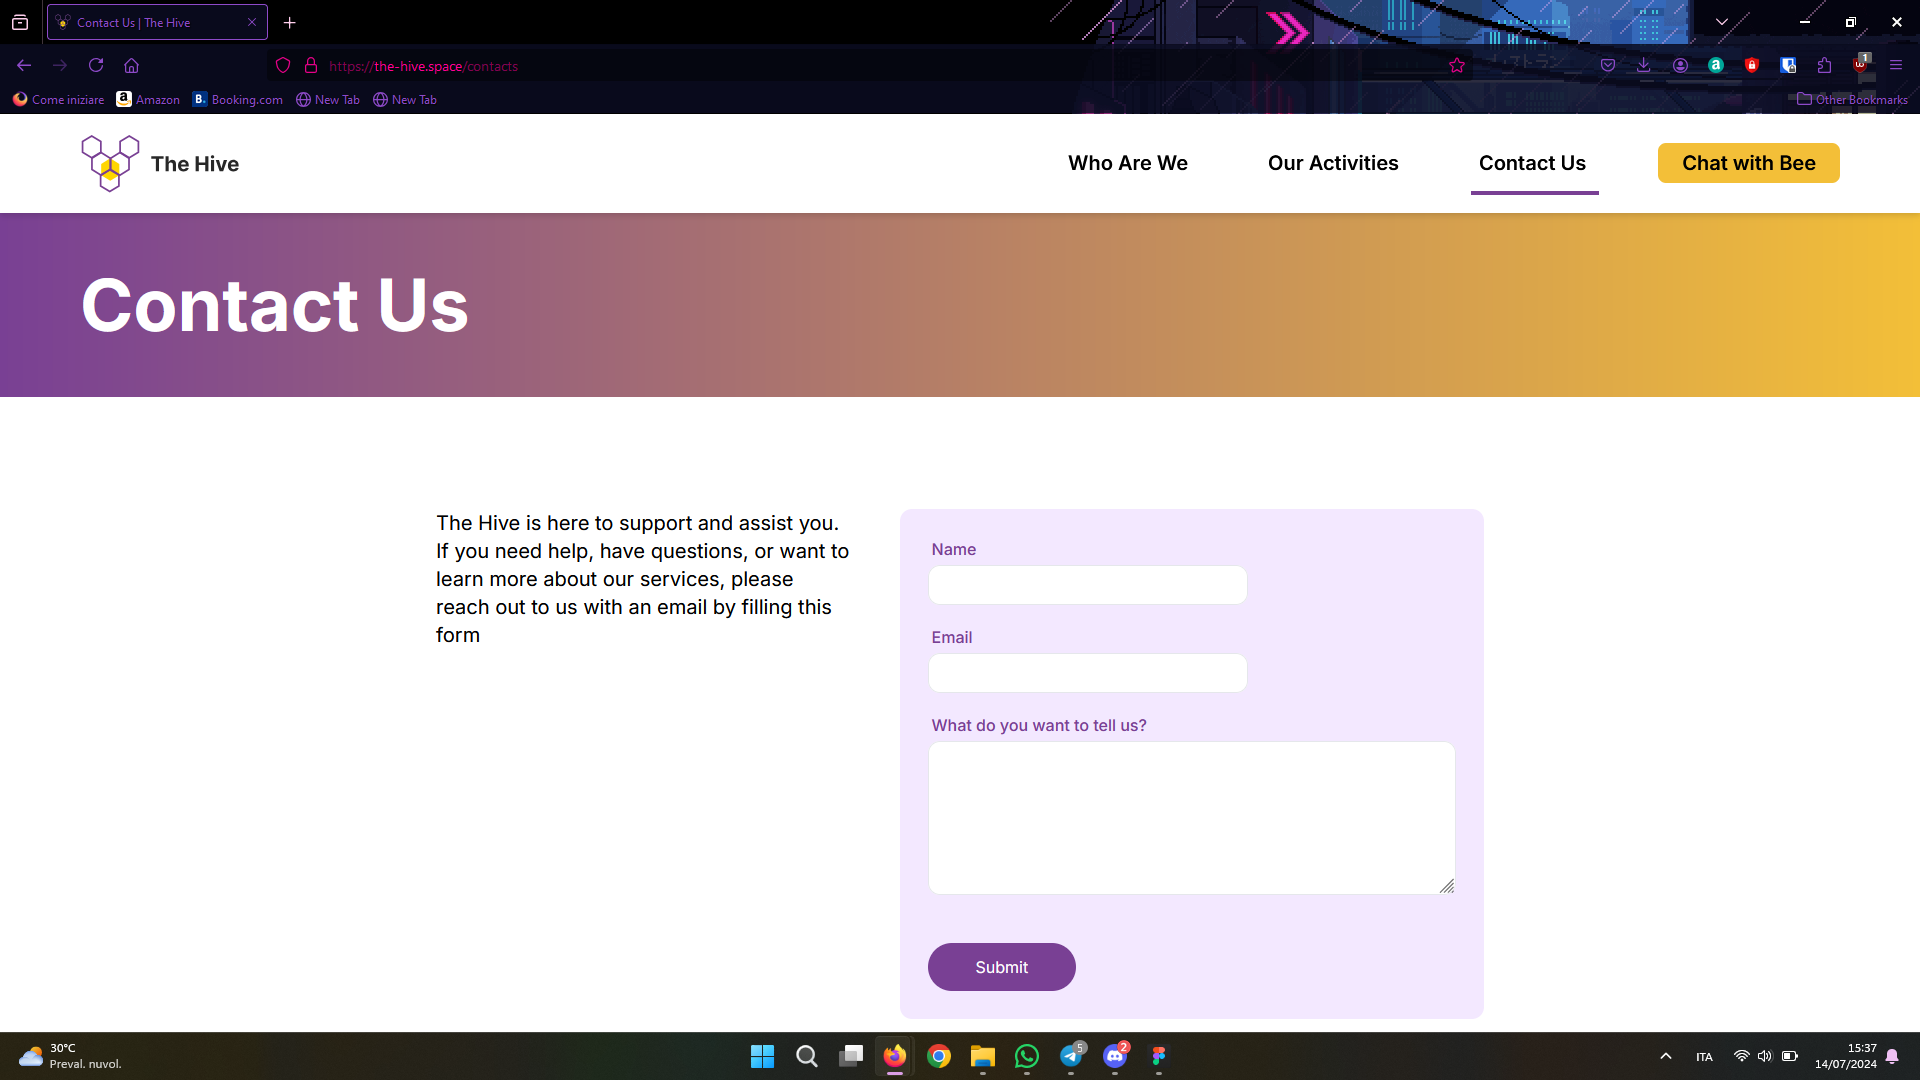
\includegraphics[width=0.5\linewidth]{img/design-document/website-screenshots/contacts.png}
\end{center}

%Chatbot
\subsection{Chatbot}
The Chatbot has its own page and has the role of being a Risk Assessor. By interacting with it, a user can figure out the severity
of a situation they're going through and receive suggestions on possible solutions or relevant contacts that they might need.
\vspace{1em}
\begin{center}
    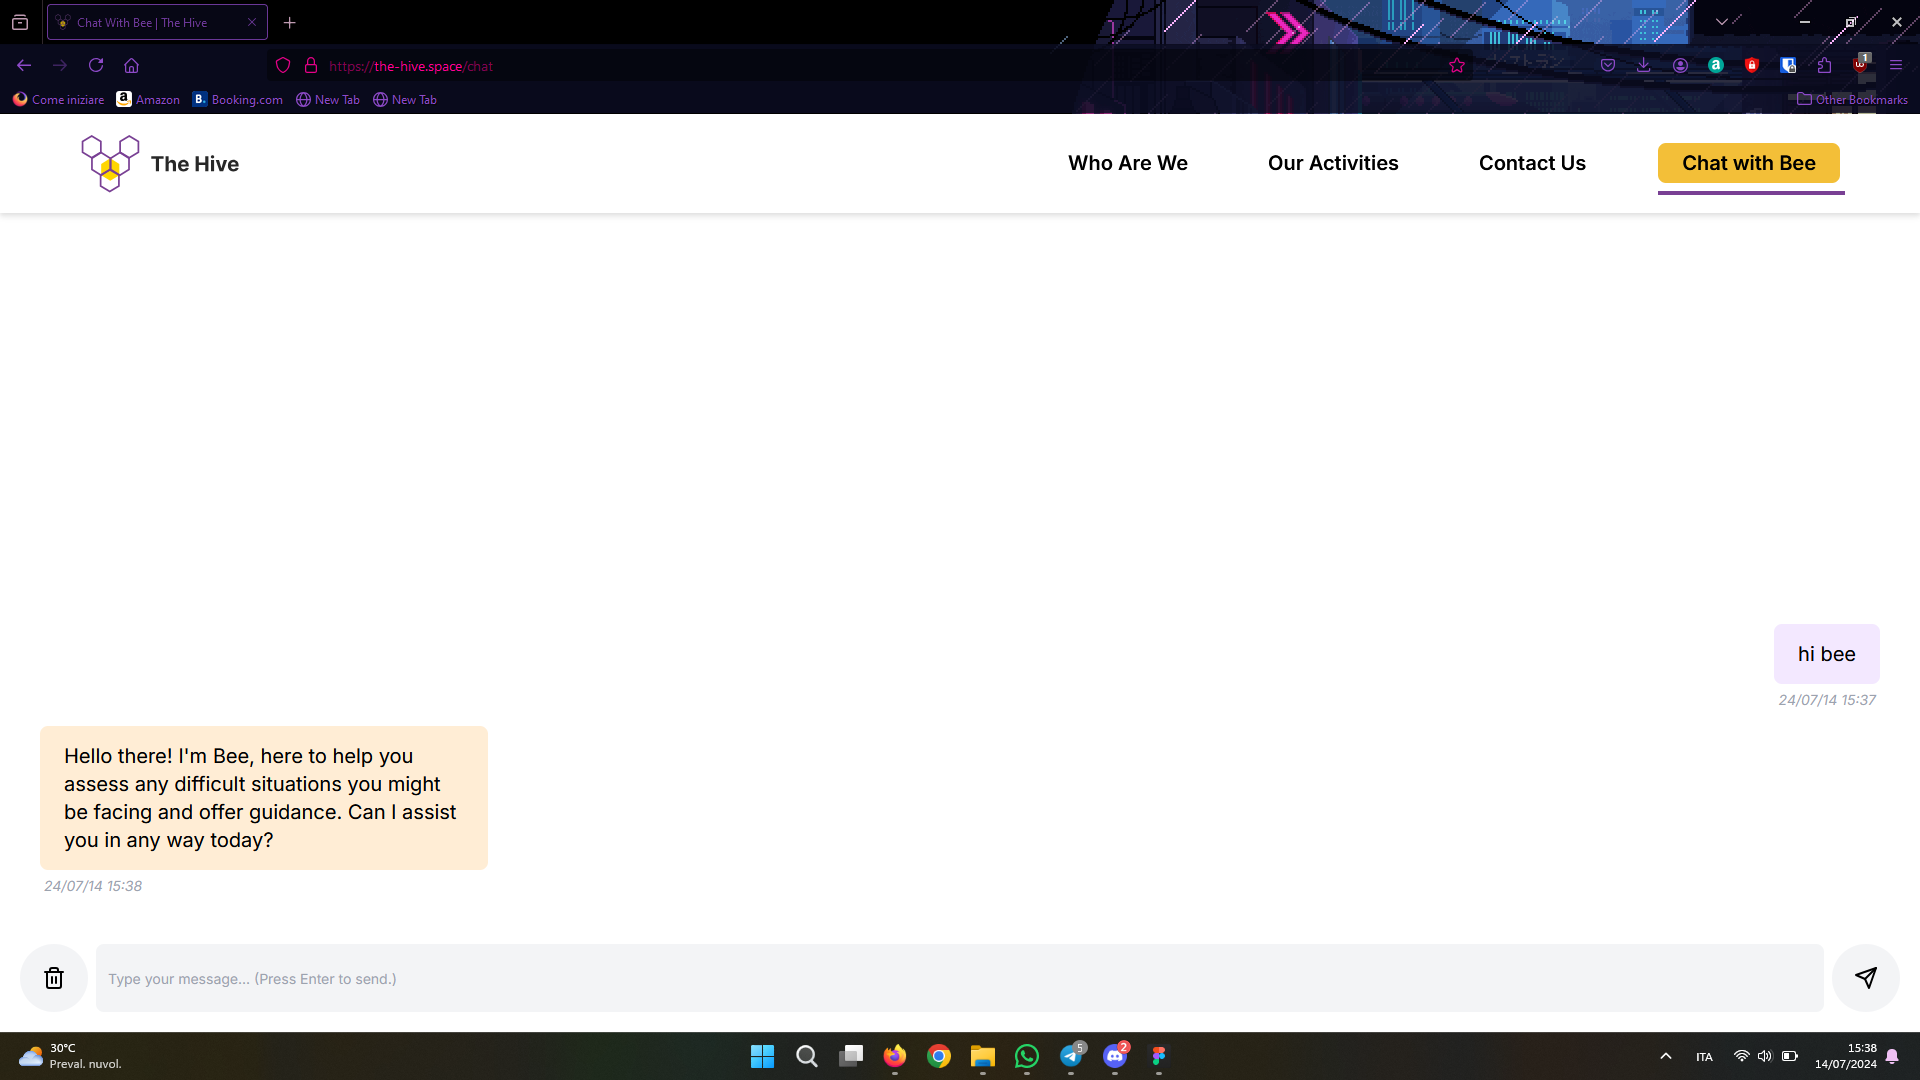
\includegraphics[width=0.5\linewidth]{img/design-document/website-screenshots/chatbot.png}
\end{center}


\pagebreak
\section{Interaction Scenarios}
We provide three interaction scenarios, considering different user persona and goals that would reflect
the typical user of the website and the execution of tasks that would be interesting for the stakeholders.


%Description
\subsection{Scenario 1}
Alessia M. is a 32 year old woman that has recently came out of an abusive relationship with her boyfriend of 7 years.
She knows that her healing process is going to take a long time and that she will need help through it.
A friend suggests her to check out The Hive, and mentions to her that the Center offers a psychological counseling service
that could help her. She starts by checking out the website: scrolling through the homepage she finds a link to the about page
of The Hive and reads through to get an idea of what the center is about. Satisfied with what she reads she uses the navigation
bar (landmarks) to find the service her friend talked to her about. Sure enough in the list of services there is the “Counseling
and Psychological Support”, she navigates to the single Service Page through the “Read More” (group link) and reads through the
additional information and testimonials, and decides to give it a try next Friday.

\vspace{2em}
%Screenshots
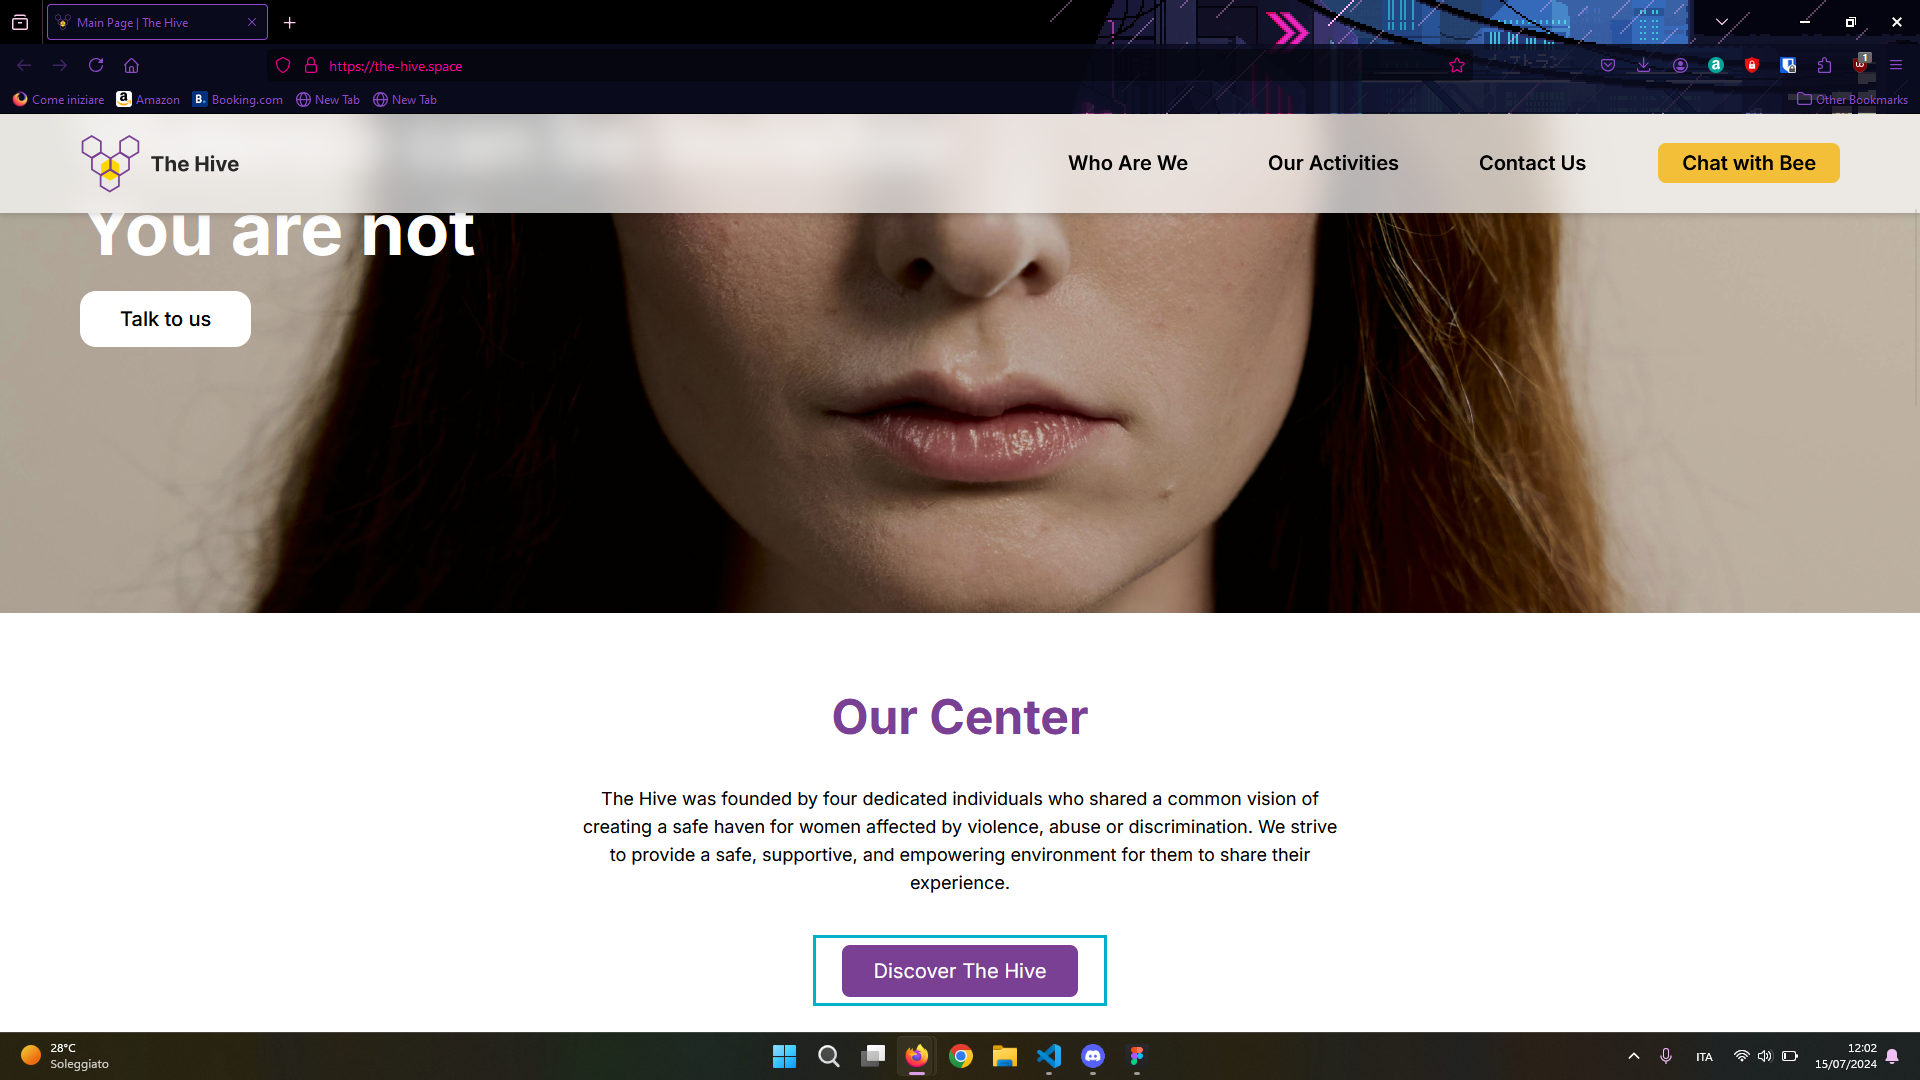
\includegraphics[width=0.5\linewidth]{img/design-document/interaction-scenarios/scenario1/step-1.png}
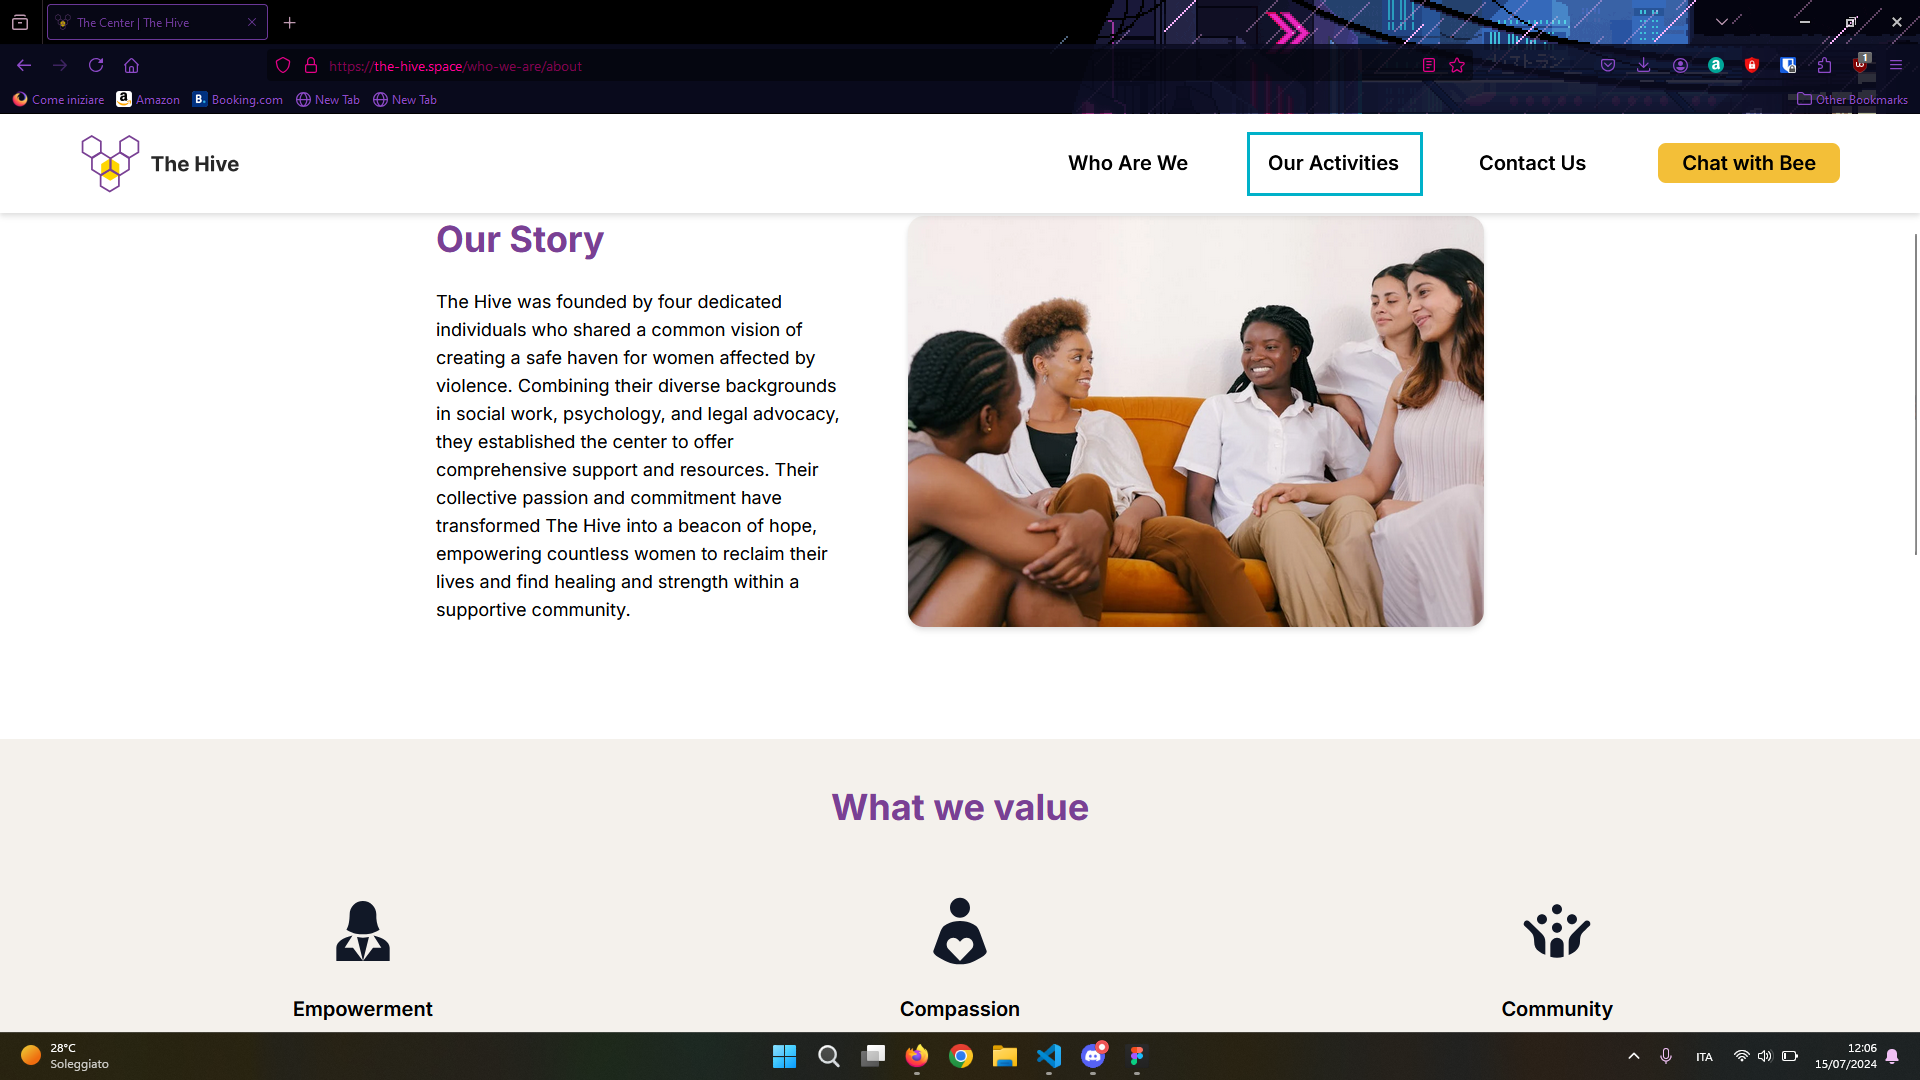
\includegraphics[width=0.5\linewidth]{img/design-document/interaction-scenarios/scenario1/step-2.png}
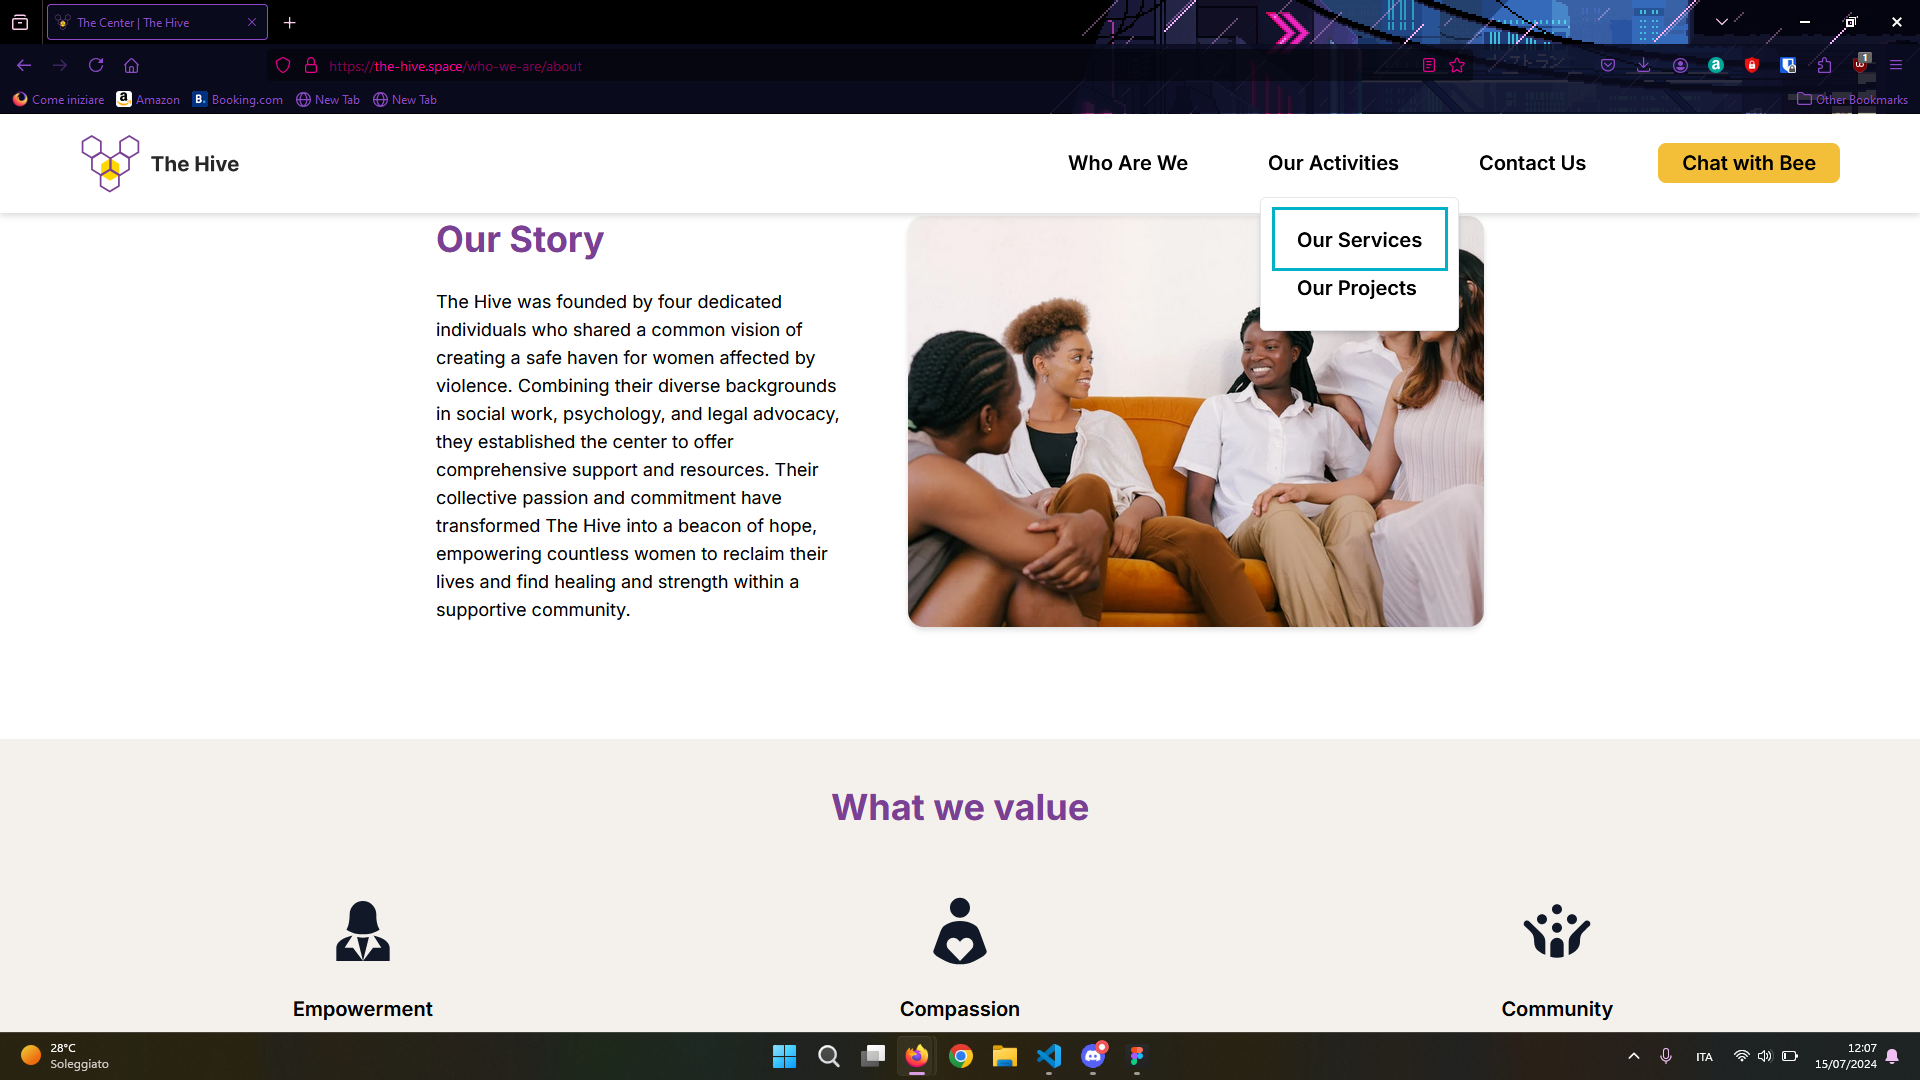
\includegraphics[width=0.5\linewidth]{img/design-document/interaction-scenarios/scenario1/step-3.png}
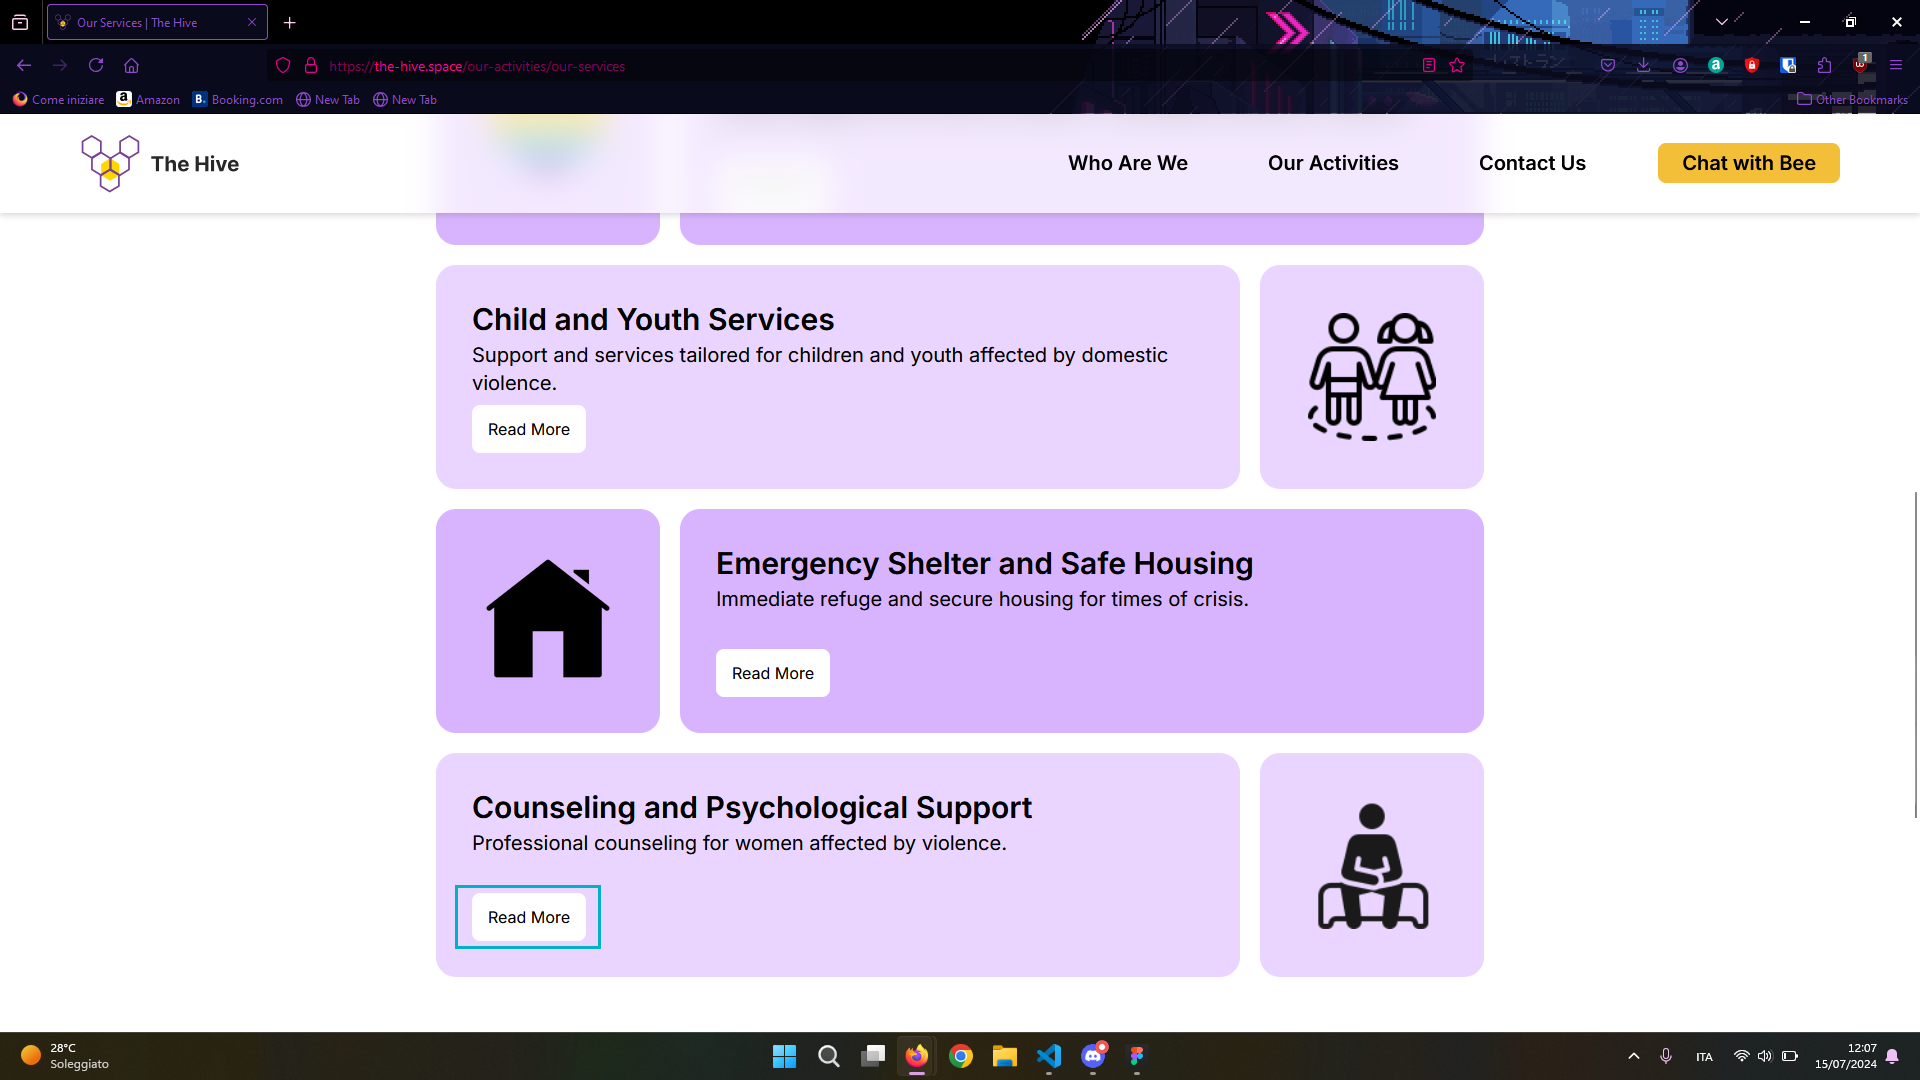
\includegraphics[width=0.5\linewidth]{img/design-document/interaction-scenarios/scenario1/step-4.png}
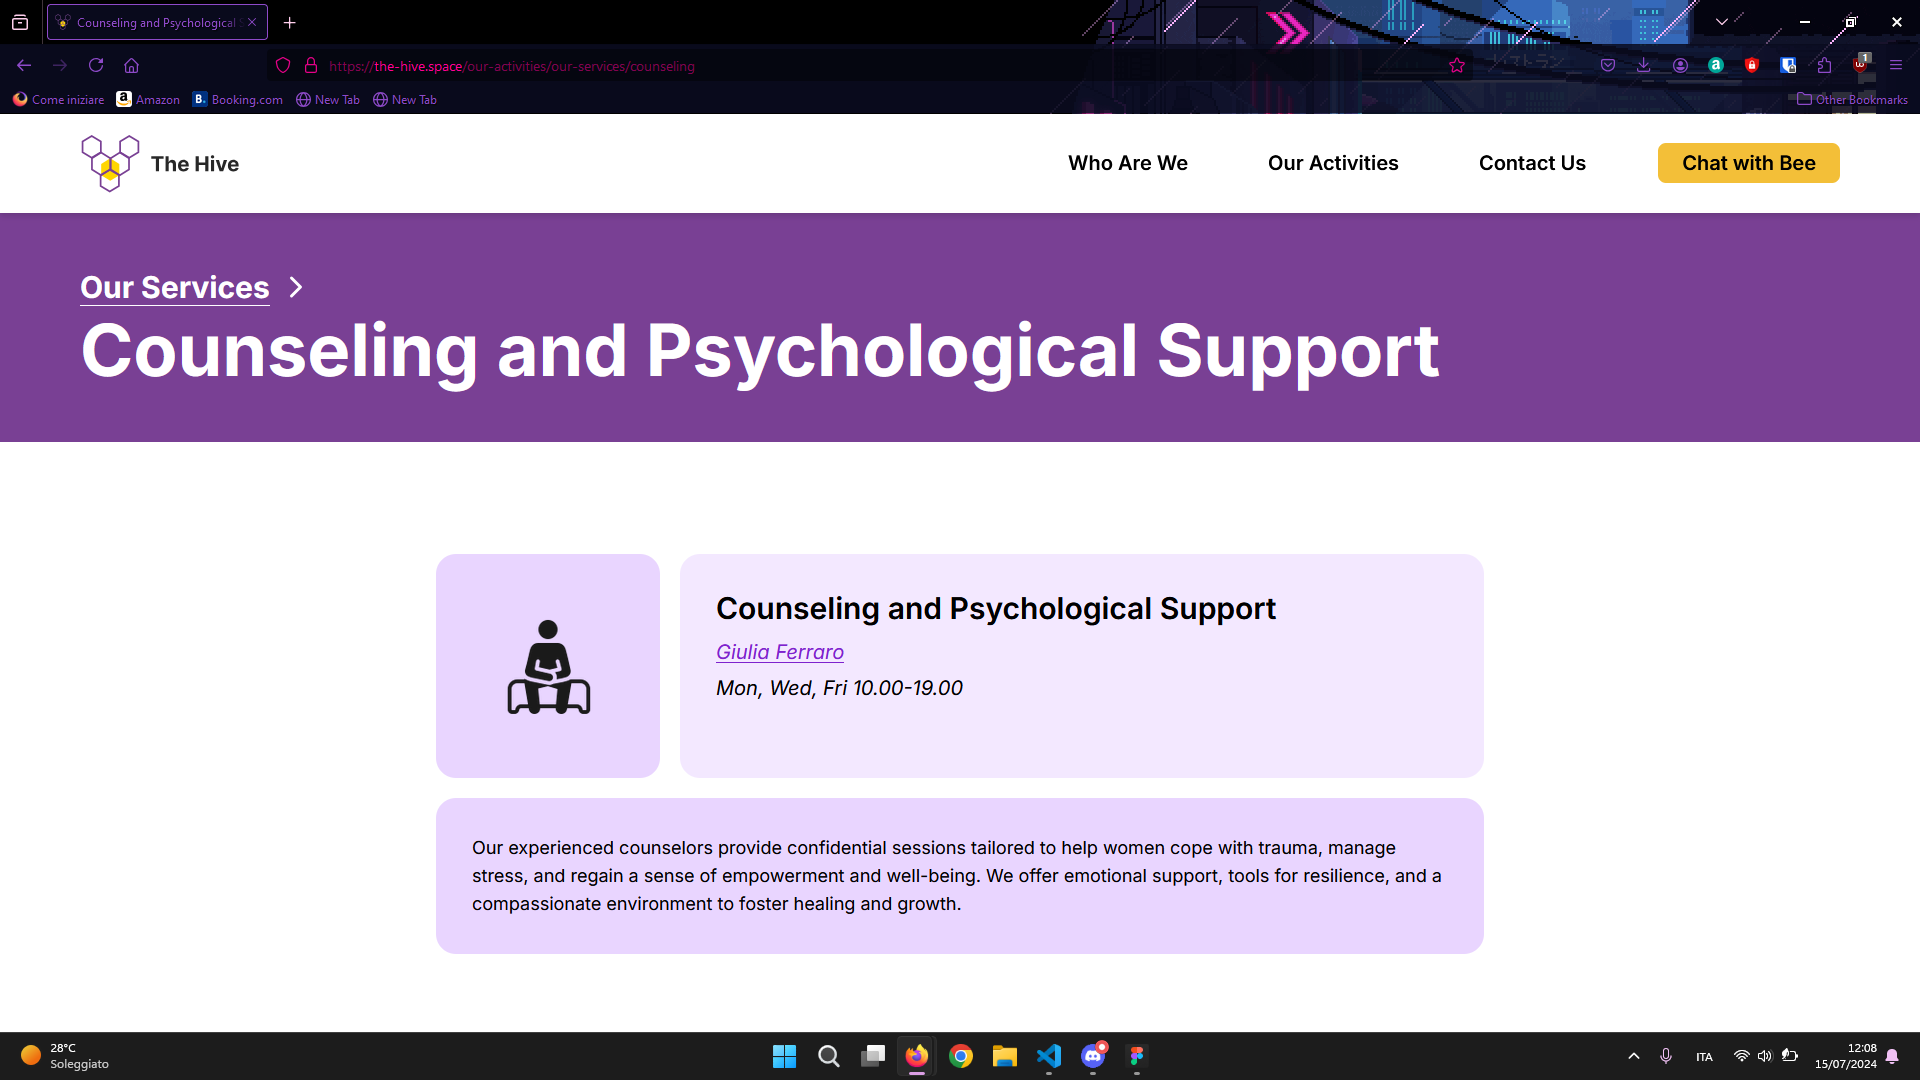
\includegraphics[width=0.5\linewidth]{img/design-document/interaction-scenarios/scenario1/step-5.png}
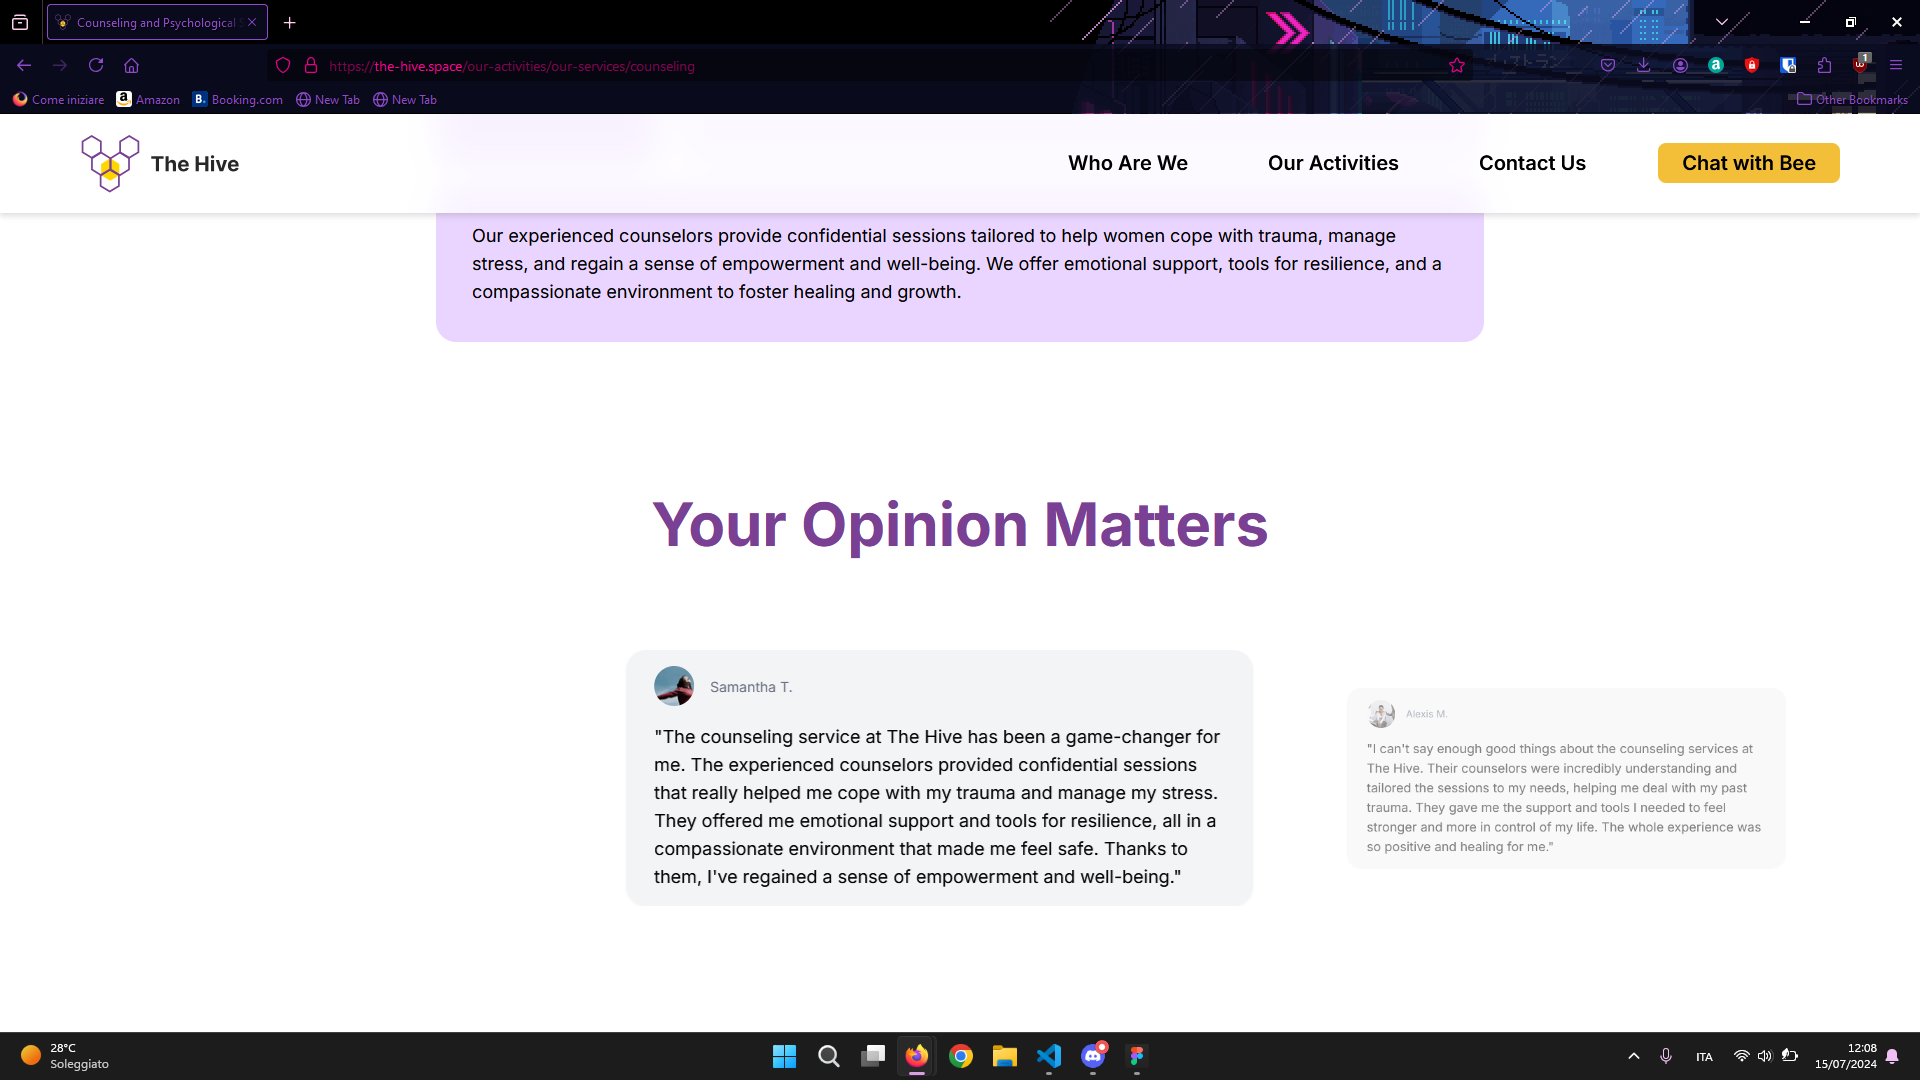
\includegraphics[width=0.5\linewidth]{img/design-document/interaction-scenarios/scenario1/step-6.png}

%Description
\subsection{Scenario 2}
A close friend of Paola S. has been struggling for some time at her workplace because of a colleague’s behavior towards here.
Paola knows that her friend has been consistently belittled and mistreated, and wants to find out how she can help her considering
the situation. She knows about The Hive and remembers that the center has recently added a risk assessing chat bot, so she decides
to try it, in order to better understand the severity of her friend's situation. Once on the homepage of the website she directly
goes for the link to the chatbot on the navigation bar (landmarks).
She chats for a bit with Bee, describing the situation of her friend and answering the questions Bee asks her.
Bee gives her a few suggestions and possible contacts that could help her friend.

\vspace{2em}
%Screenshots
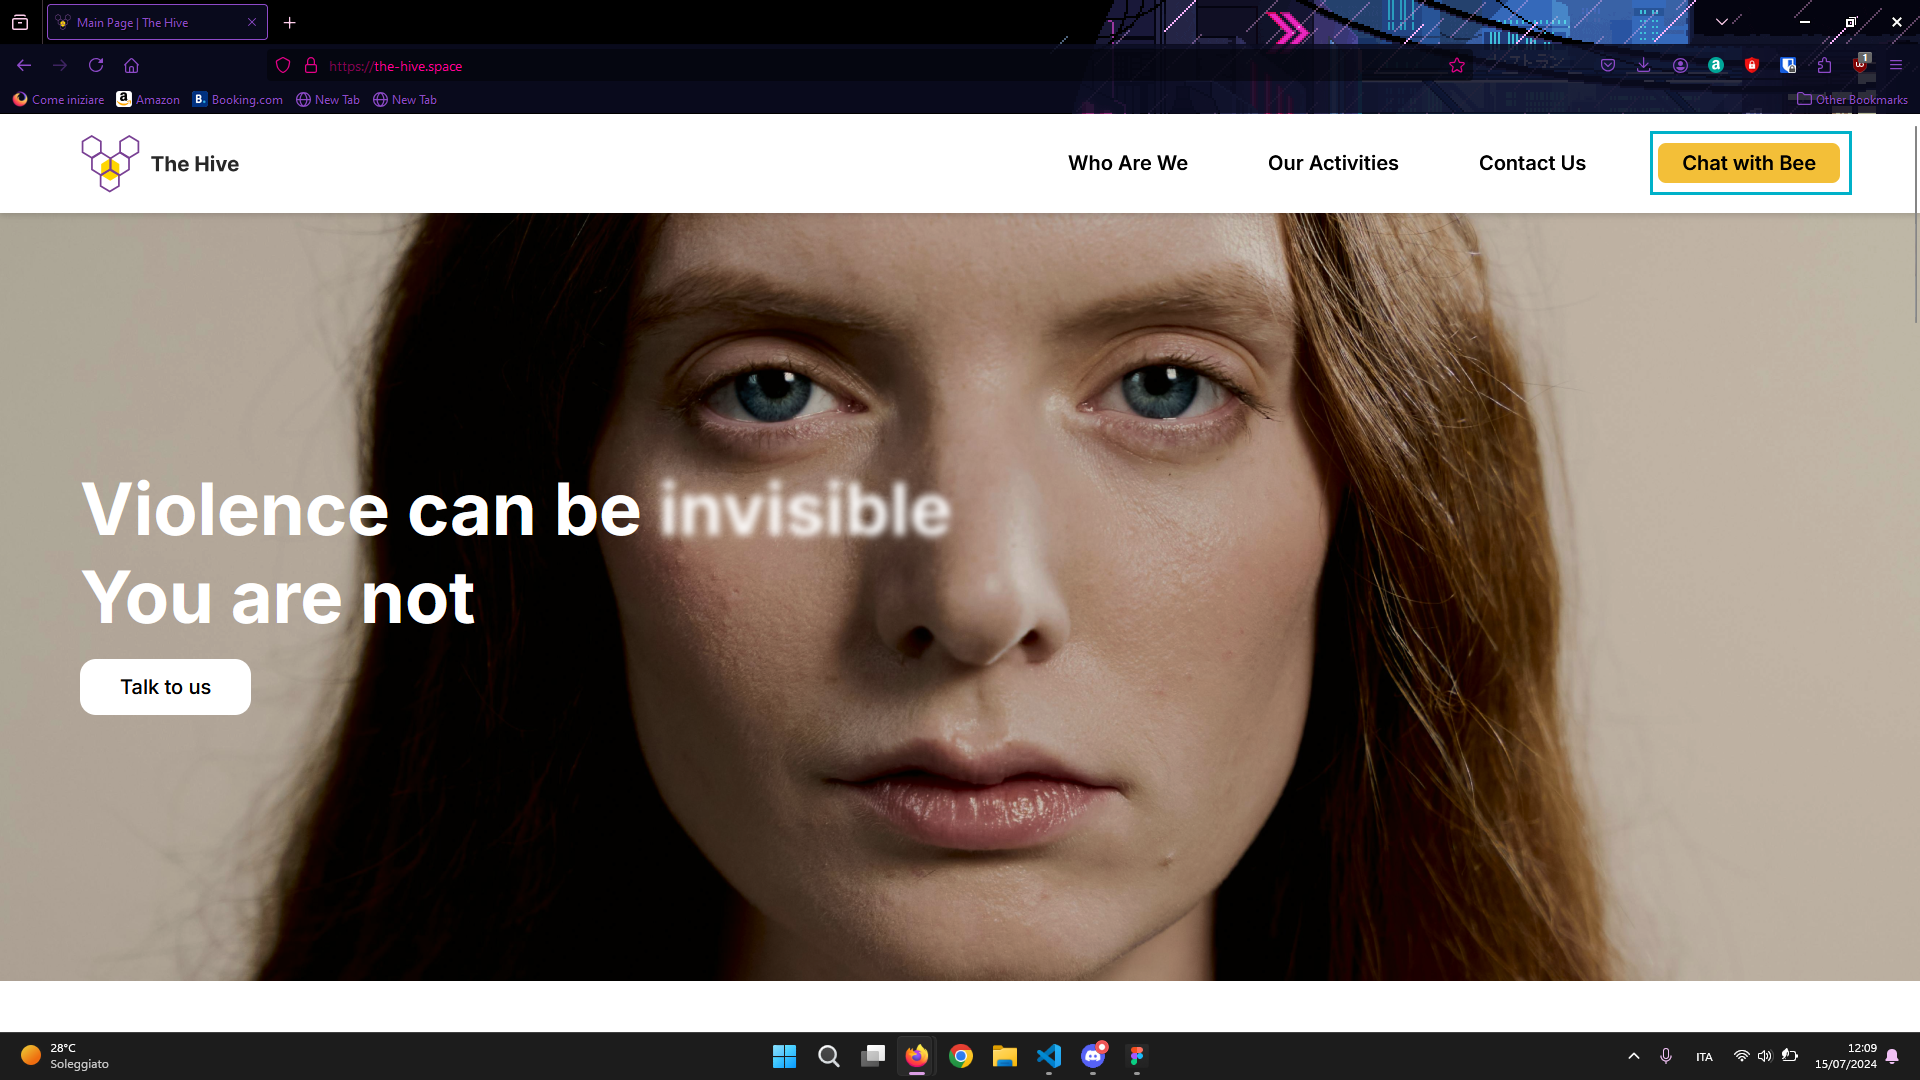
\includegraphics[width=0.5\linewidth]{img/design-document/interaction-scenarios/scenario2/step-1.png}
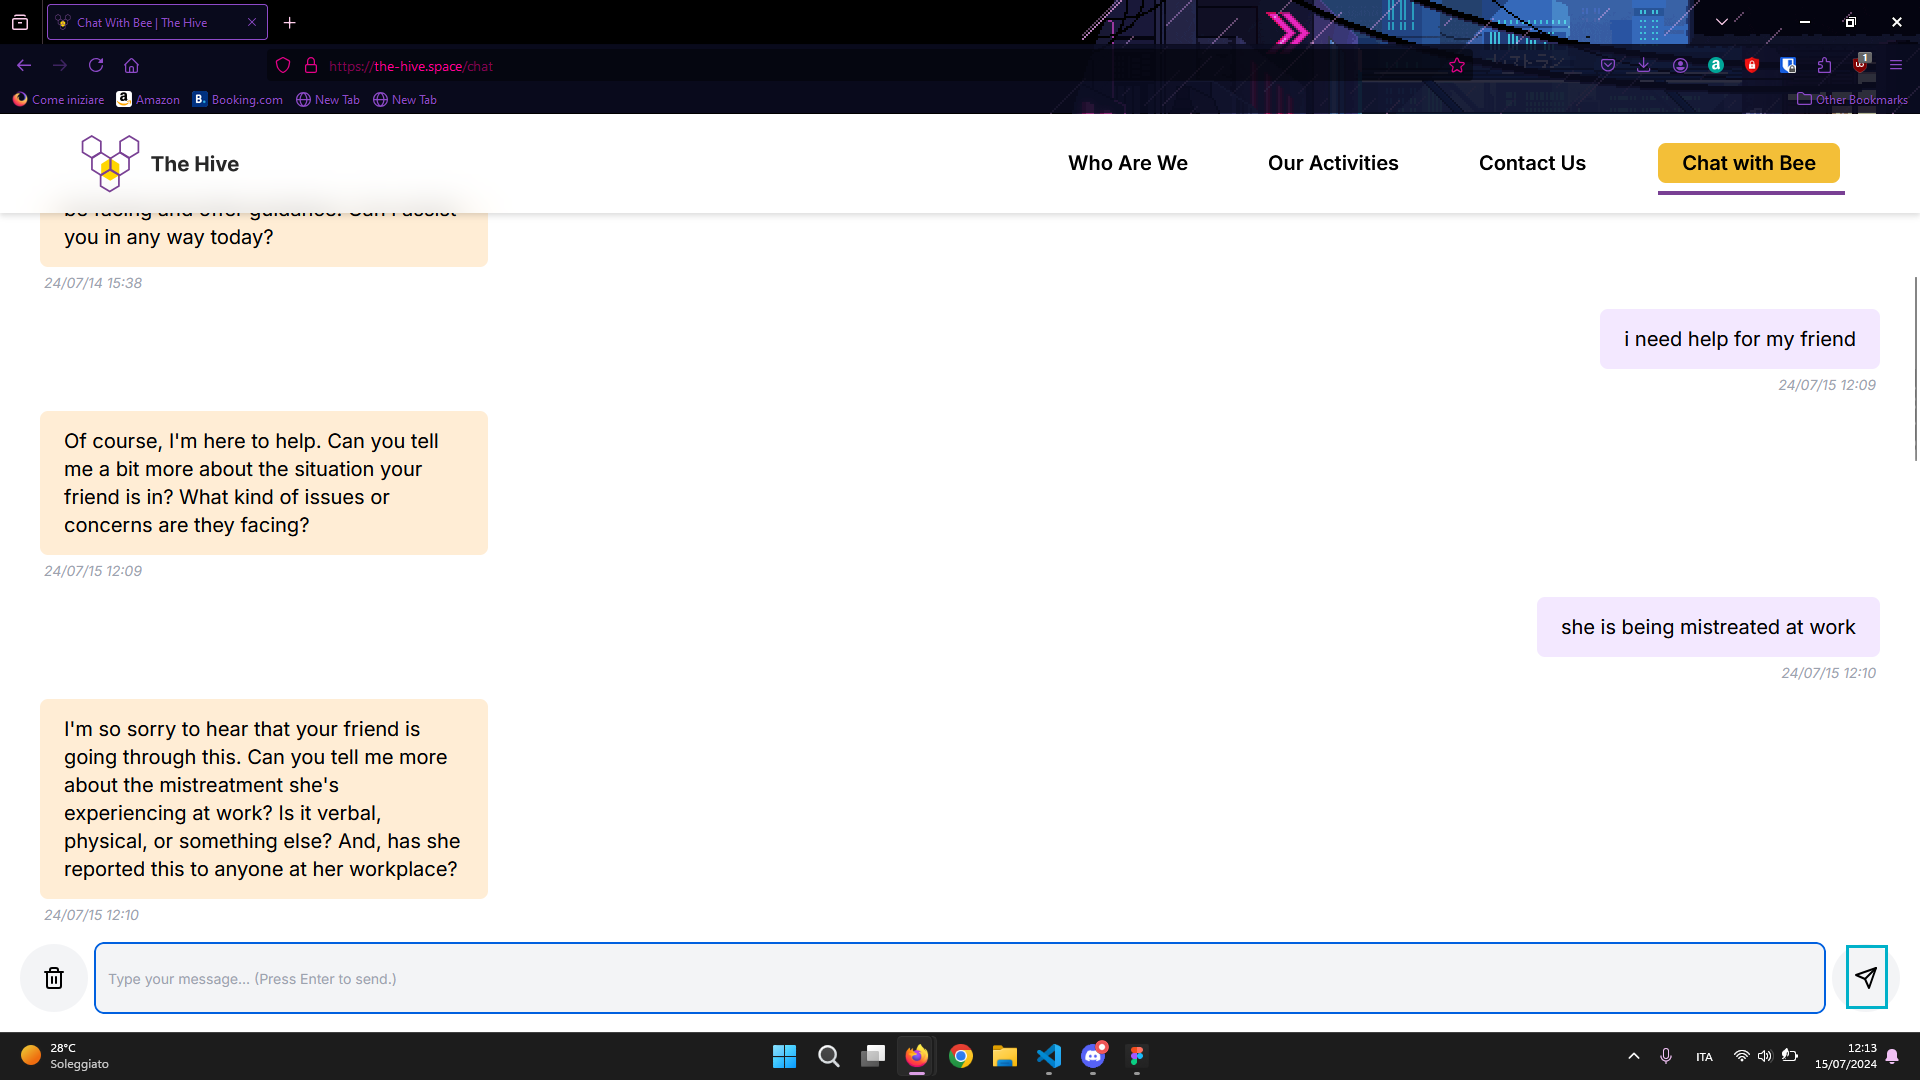
\includegraphics[width=0.5\linewidth]{img/design-document/interaction-scenarios/scenario2/step-2.png}

%Description
\subsection{Scenario 3}
Giovanni L. is the principal of a middle school based in Milan. Recently one of the teachers in his school has mentioned that she
wanted to organize a seminar to sensitize the students about the topic of gender inequality for the occasion of the International
Women’s day. For this purpose she gave him the name of a contact she knows from the center The Hive.  Giovanni goes into the center’s
website and through the navigation bar (landmarks) he easily finds the “Who we are” page. Here he browses to find “Filippo Pantaleone”
(group link), the contact of his colleague, and looks through his Profile page. Utilizing the sidebar links (structural links) he finds
the activities Filippo is responsible for and follows the link to the project “ARYA, To Counter Gender Stereotypes”, which is perfect for
what he’s looking for. He decides then to contact the center through the apposite section on the website.

\vspace{2em}
%Screenshots
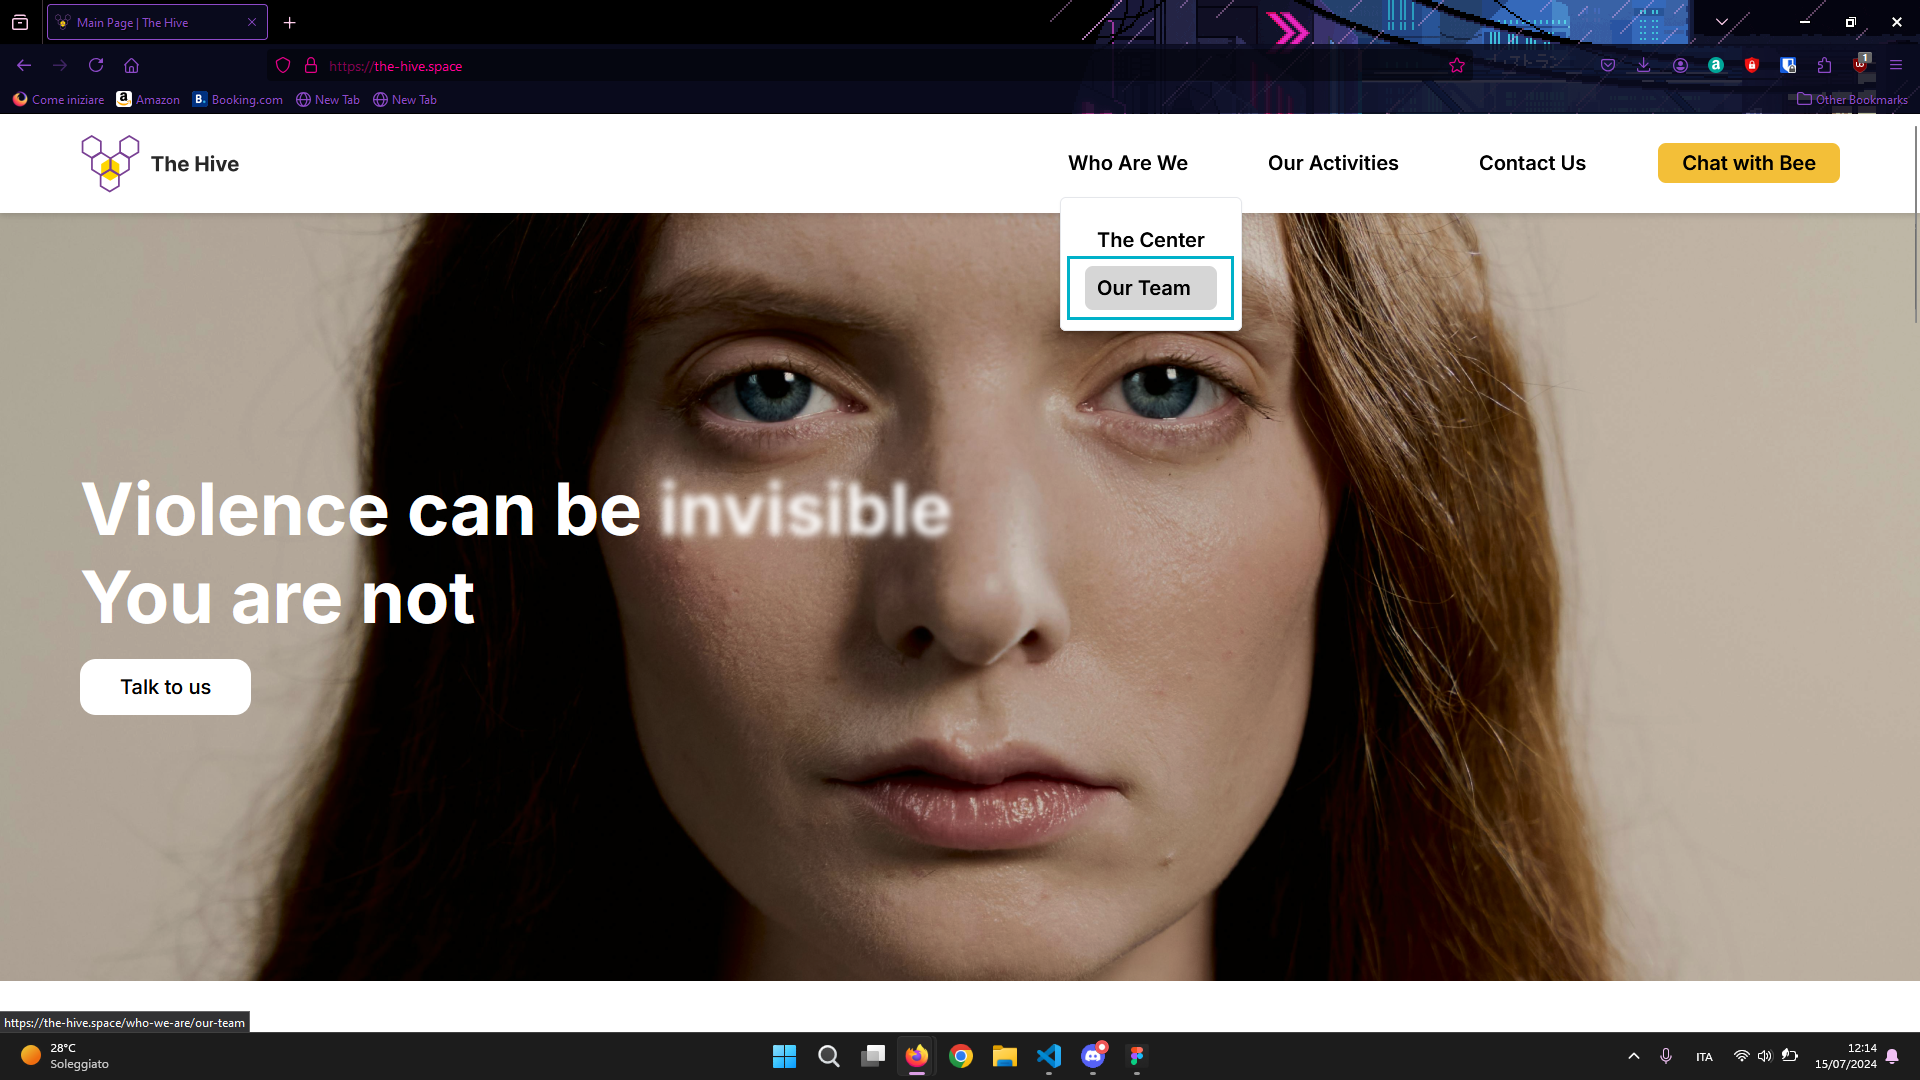
\includegraphics[width=0.5\linewidth]{img/design-document/interaction-scenarios/scenario3/step-1.png}
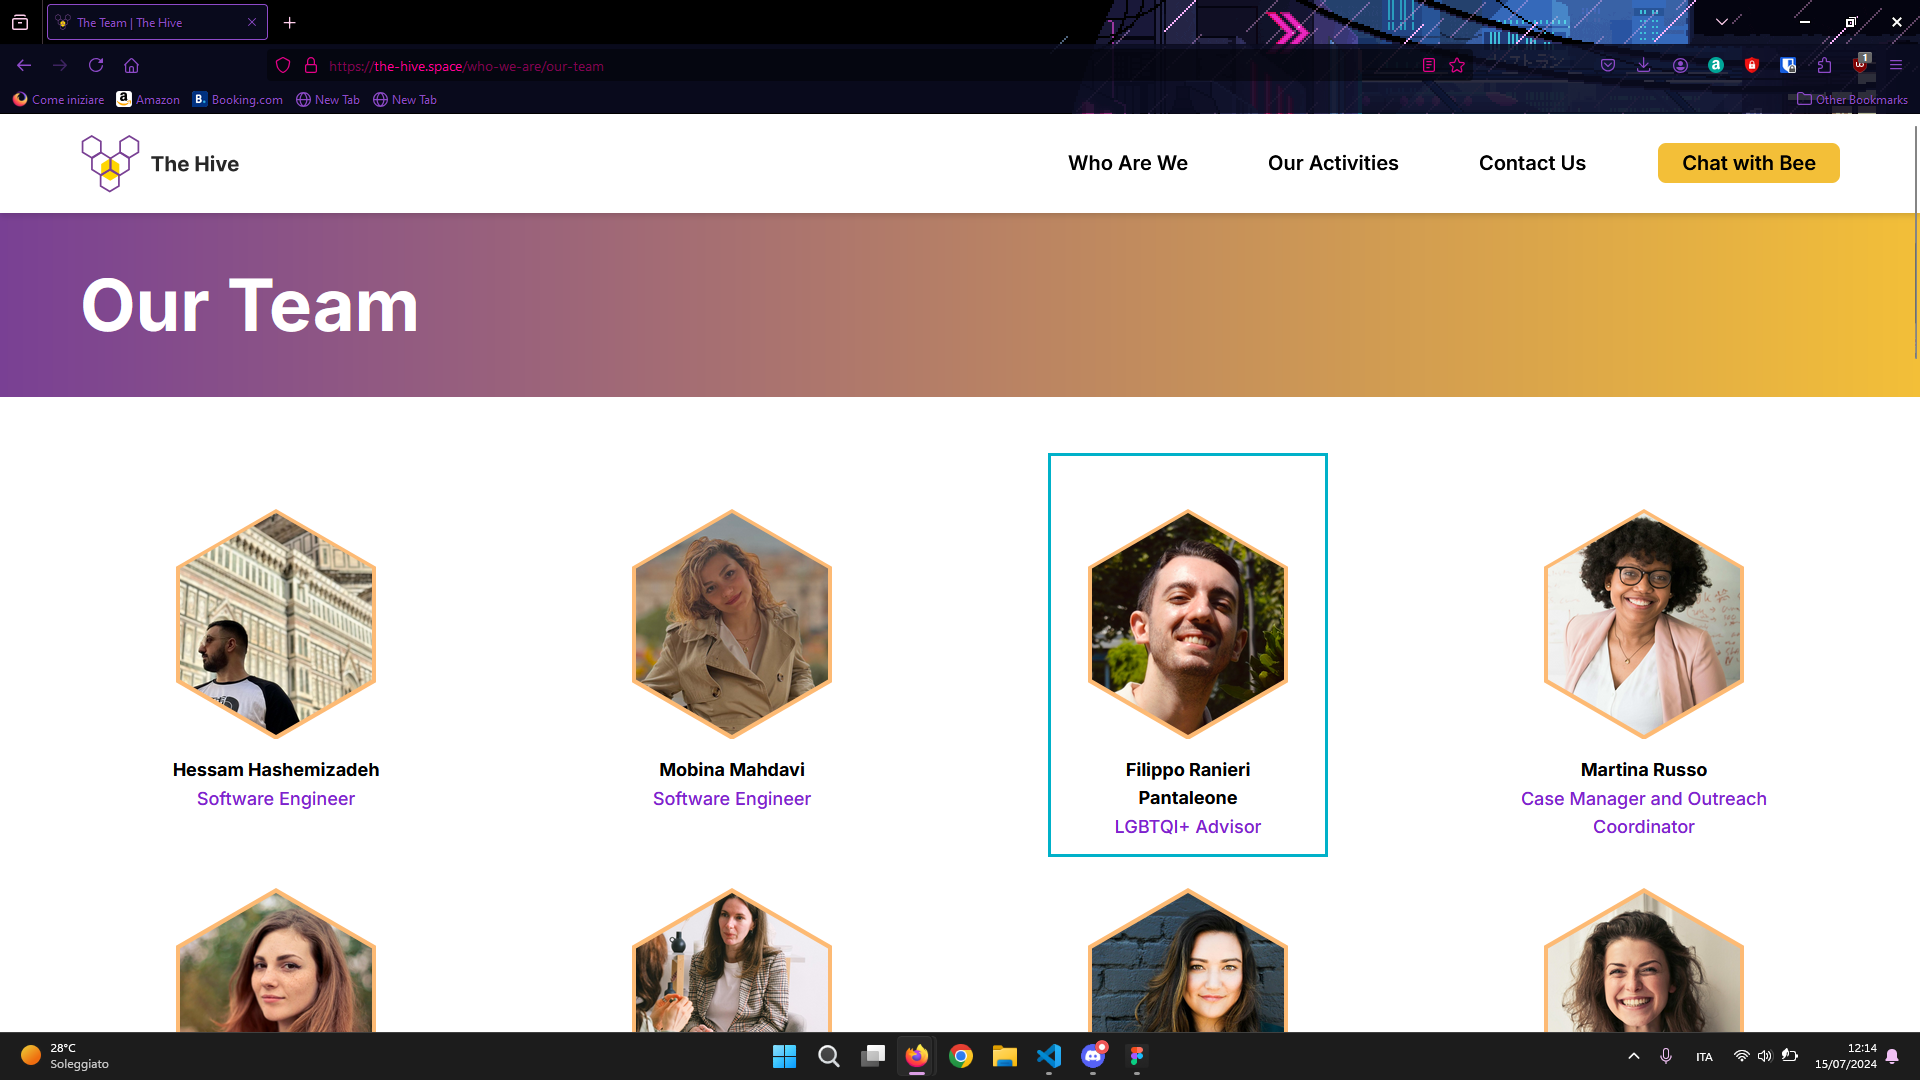
\includegraphics[width=0.5\linewidth]{img/design-document/interaction-scenarios/scenario3/step-2.png}
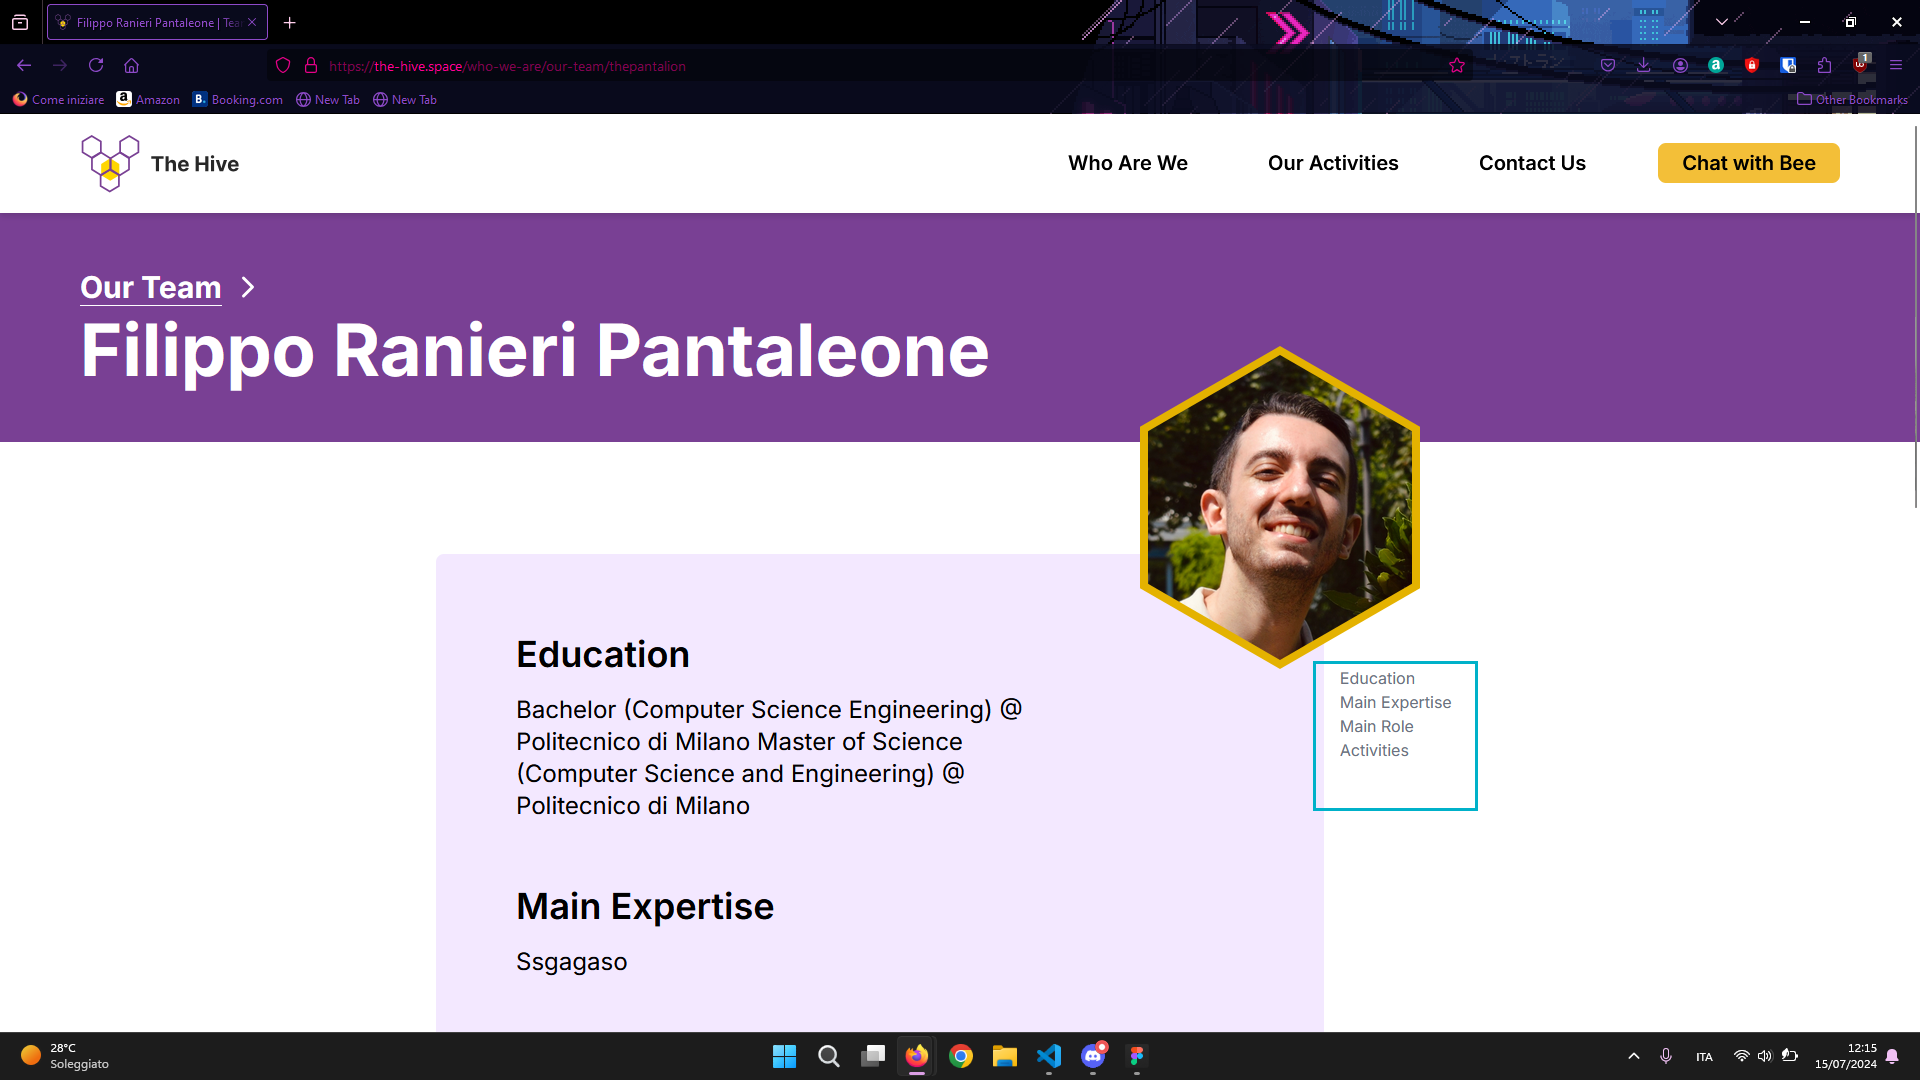
\includegraphics[width=0.5\linewidth]{img/design-document/interaction-scenarios/scenario3/step-3.png}
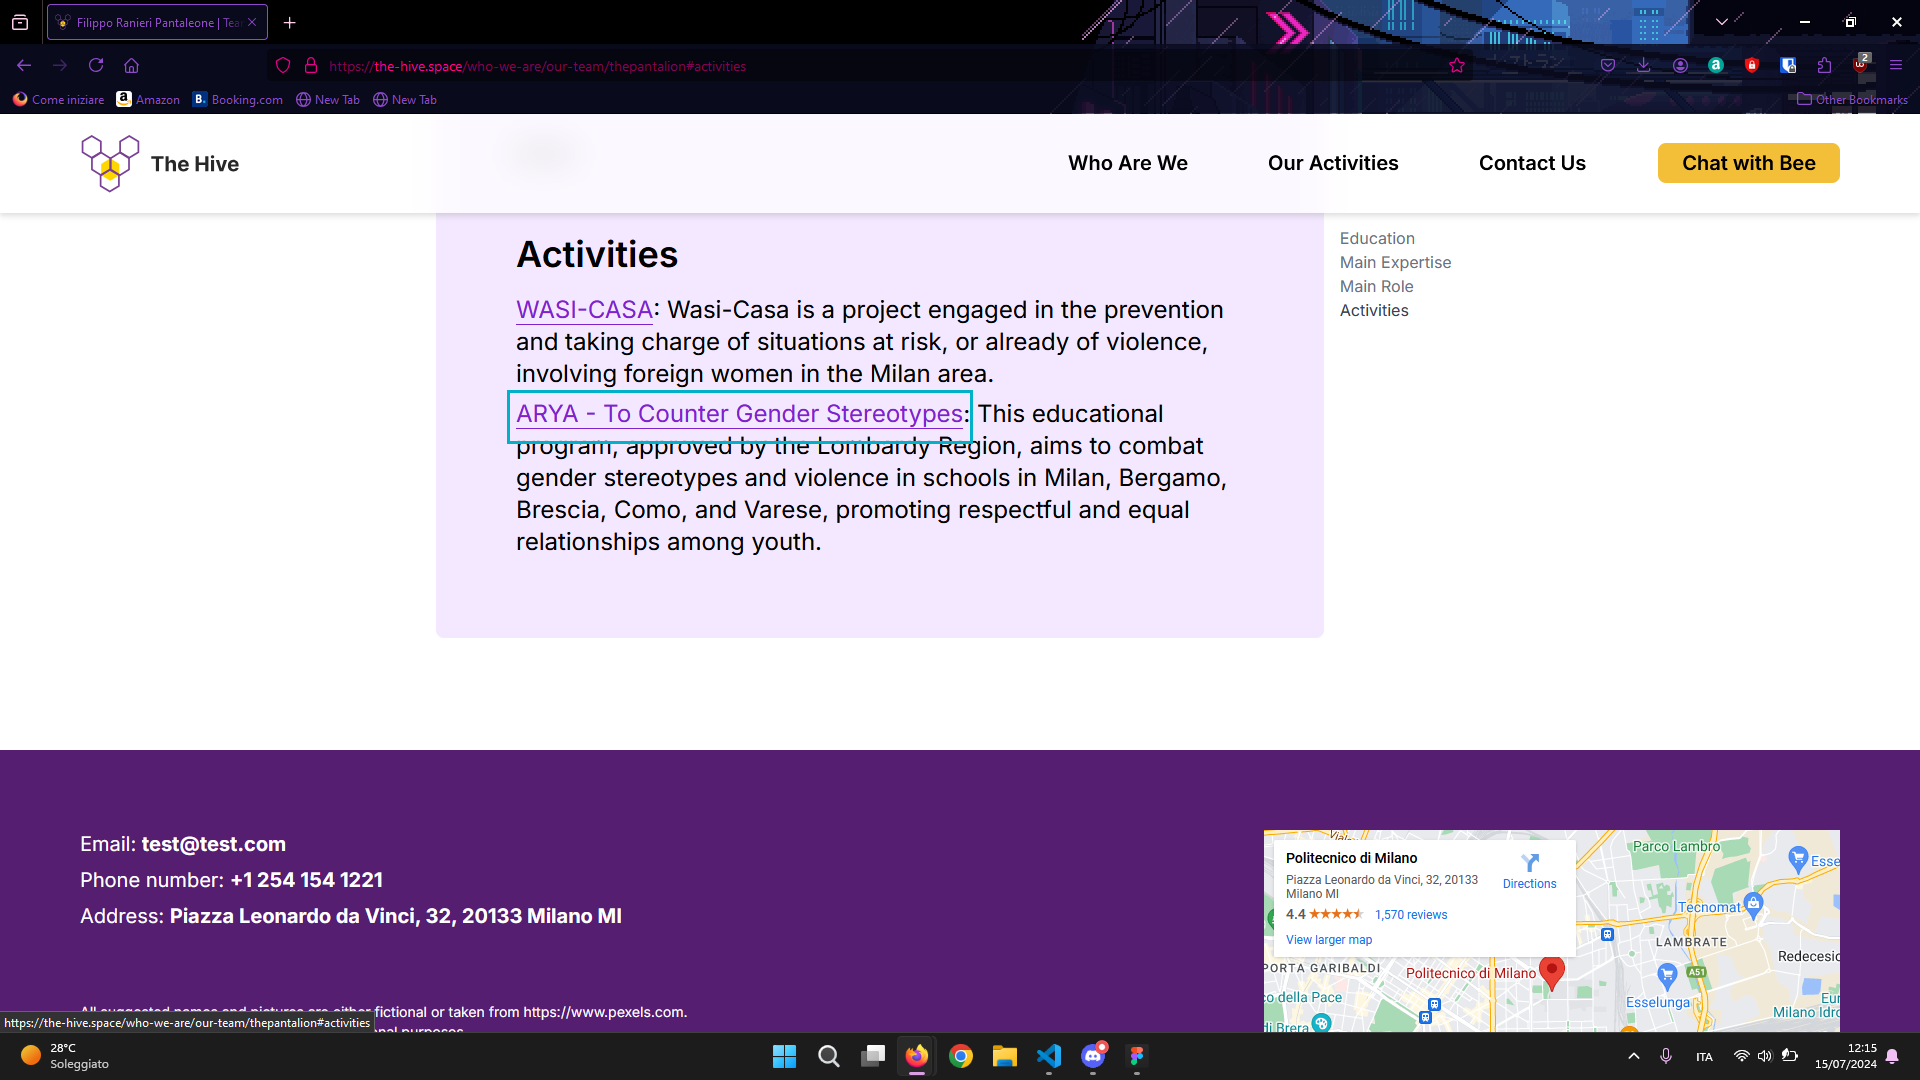
\includegraphics[width=0.5\linewidth]{img/design-document/interaction-scenarios/scenario3/step-4.png}
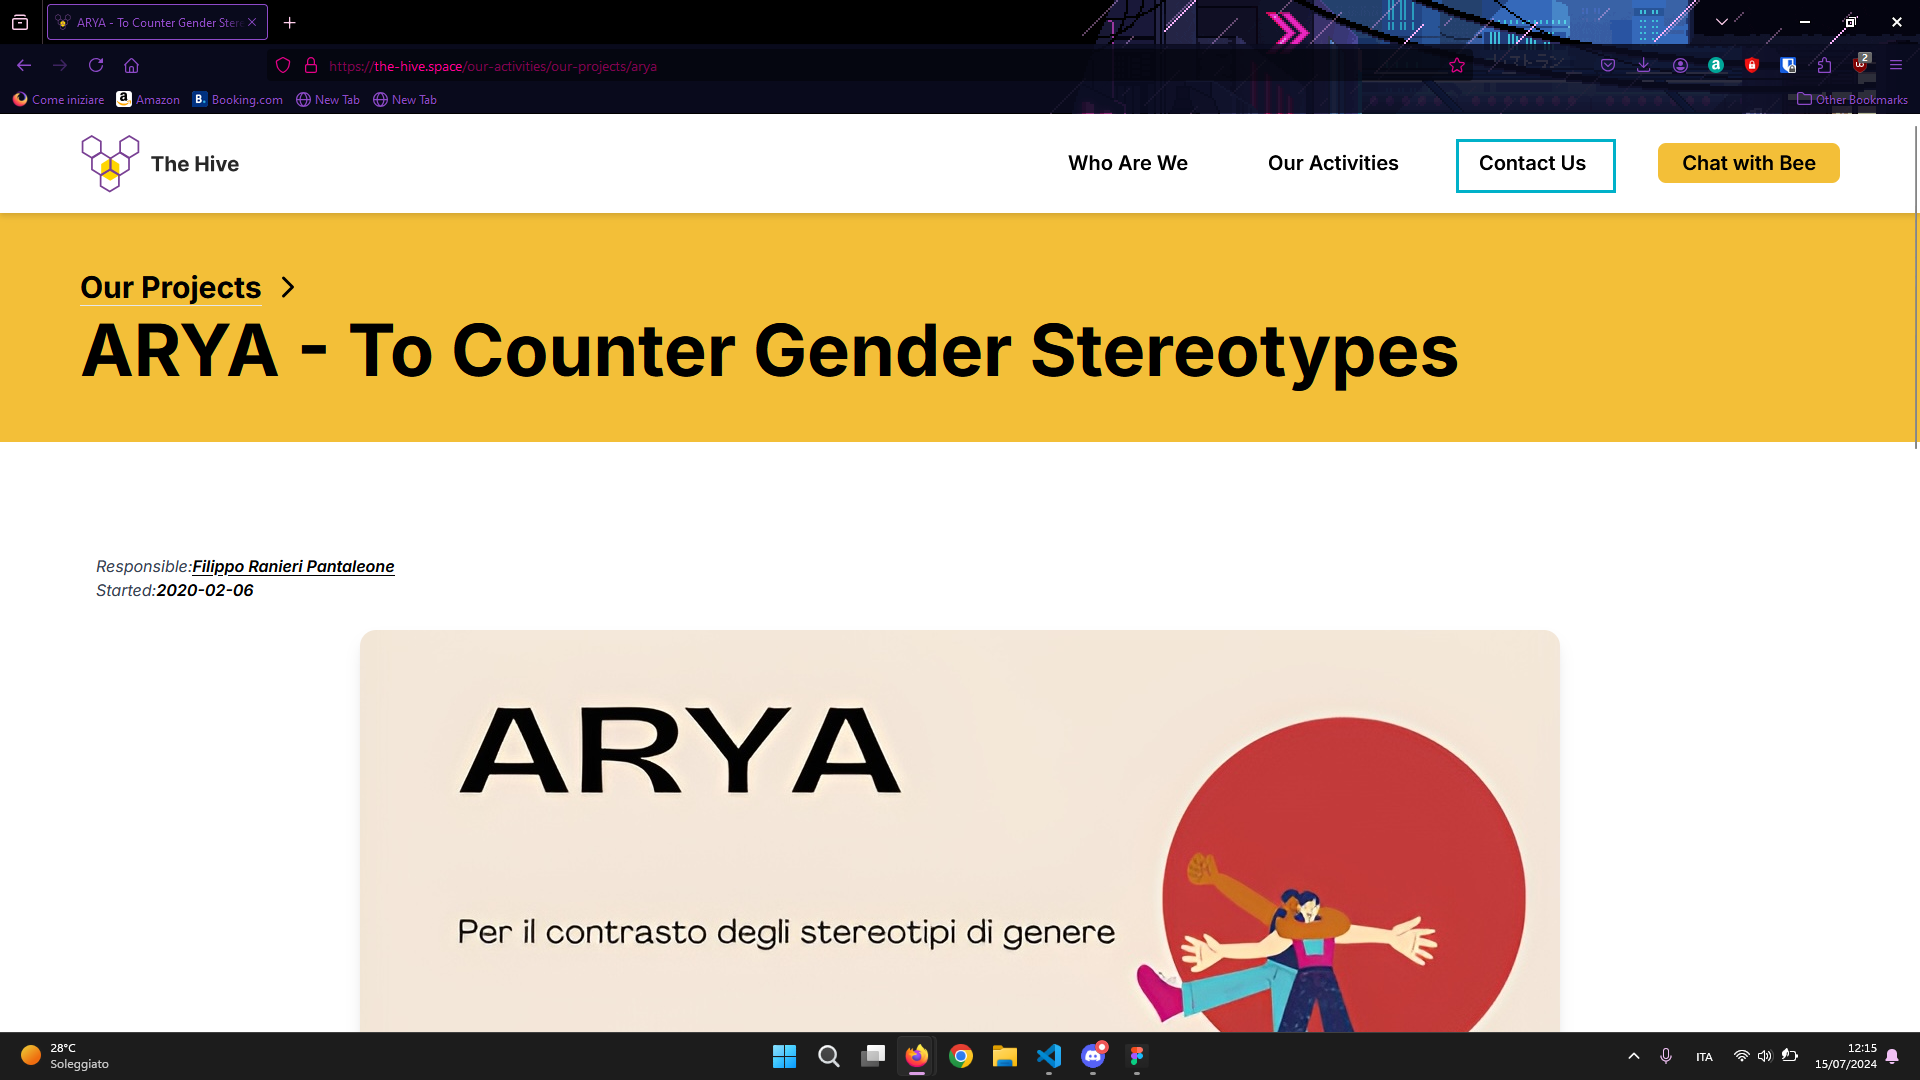
\includegraphics[width=0.5\linewidth]{img/design-document/interaction-scenarios/scenario3/step-5.png}
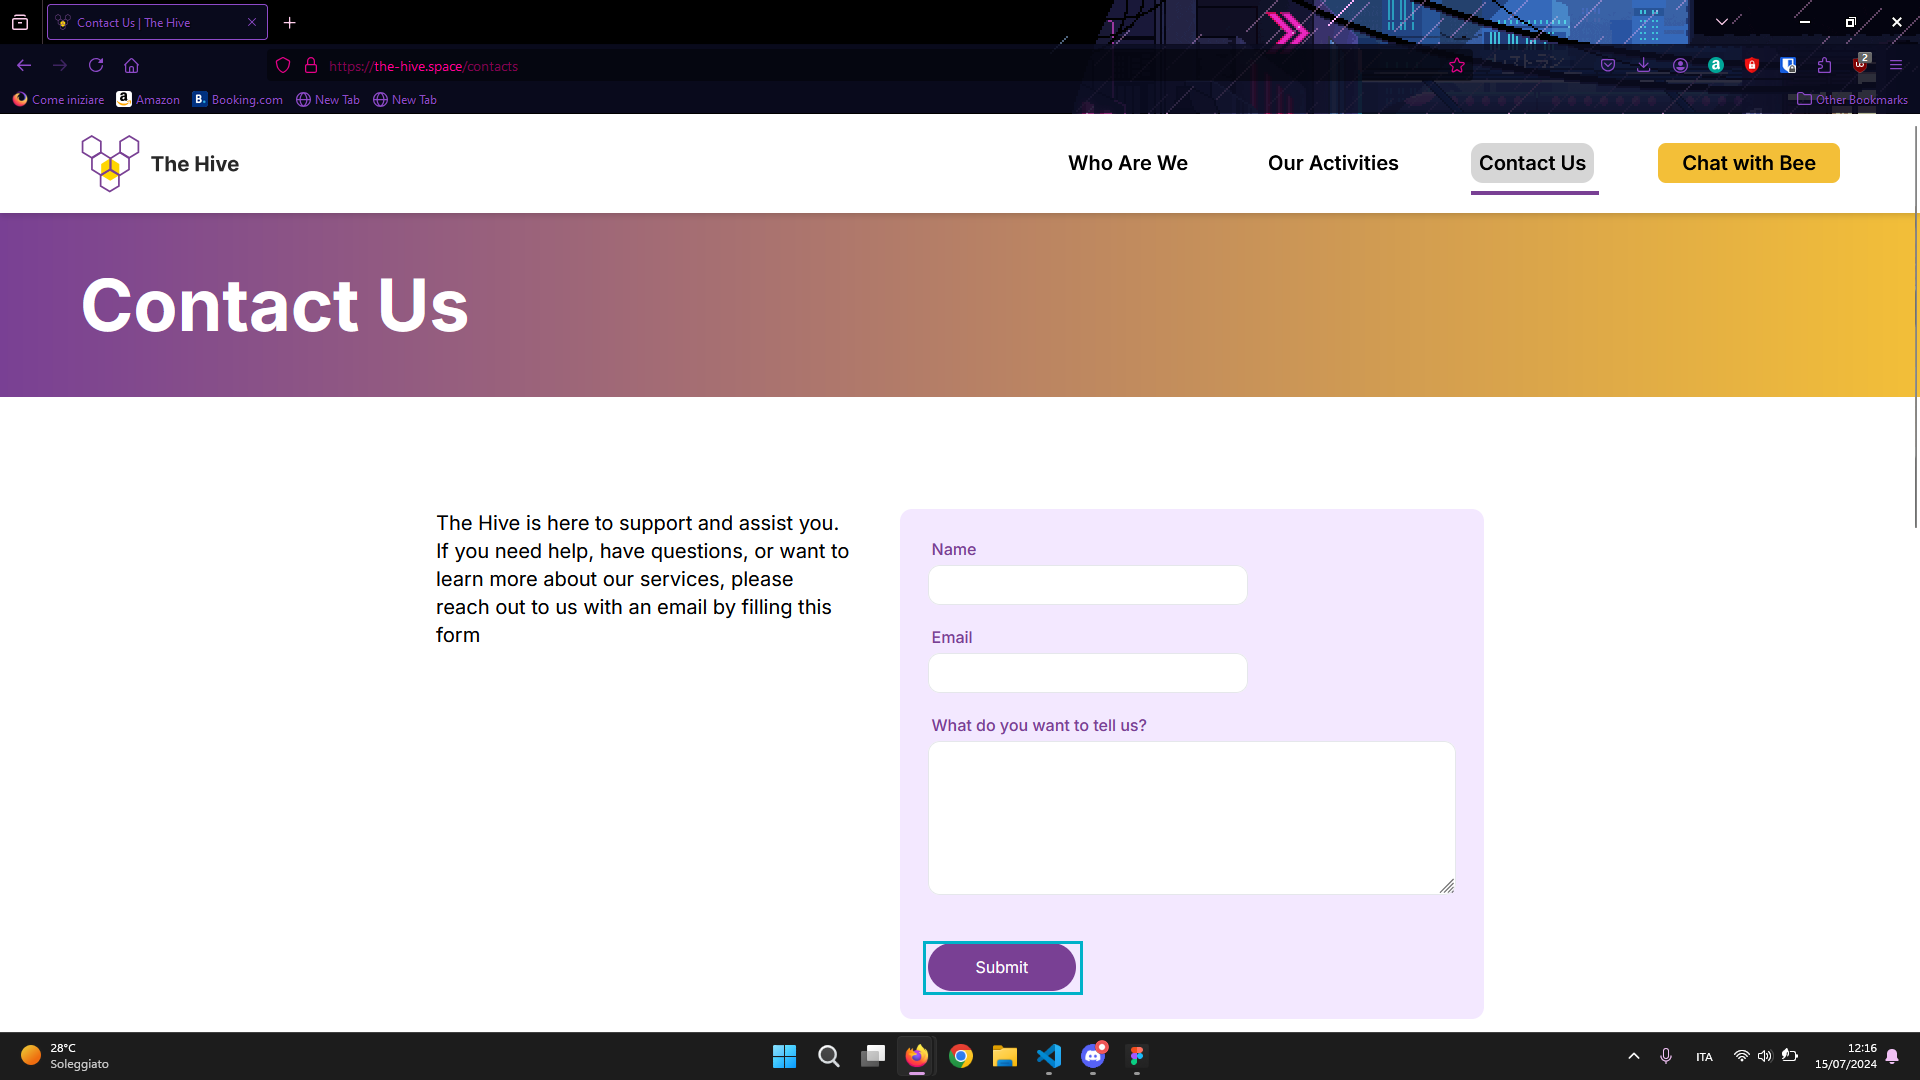
\includegraphics[width=0.5\linewidth]{img/design-document/interaction-scenarios/scenario3/step-6.png}


\pagebreak
\section{DB Design}
\subsection{ER Schema}

% TODO Verify that all design steps are included here
